\documentclass[12pt,a4paper,oneside]{report}

% ---------------------------------------------------------------- packages
\usepackage[utf8]{inputenc}
\usepackage[T1]{fontenc}
\usepackage{lmodern}
\usepackage[top=2.3cm,bottom=2.3cm,left=2.5cm,right=2.2cm]{geometry}
\usepackage{setspace}
\usepackage{graphicx}
\usepackage{float}
\usepackage{booktabs}
\usepackage{tabularx}
\usepackage{array}
\usepackage{longtable}
\usepackage{multirow}
\usepackage[table]{xcolor}
\usepackage{amsmath}
\usepackage{enumitem}
\usepackage{caption}
\usepackage{subcaption}
\usepackage{listings}
\usepackage{fancyhdr}
\usepackage{titlesec}
\usepackage{tikz}
\usetikzlibrary{shapes.geometric,shapes.multipart,arrows.meta,positioning,fit,calc,backgrounds}
\usepackage[hidelinks]{hyperref}

% =====================================================================
%  EDIT THESE LINES ONLY - used by both the report and the slides.
%  After editing, recompile (see docs/README.md).
% =====================================================================
\newcommand{\ProjectTitle}{SmartDock: A Multi-Tenant Dock Appointment Scheduling and Yard Management System for Warehouses and Distribution Centres}
\newcommand{\ProjectShortTitle}{SmartDock}
\newcommand{\StudentName}{[Student Name]}
\newcommand{\RegisterNumber}{[Register Number]}
\newcommand{\GuideName}{[Guide Name, Designation]}
\newcommand{\Programme}{[Programme, e.g. MBA / B.Tech]}
\newcommand{\Department}{[Department Name]}
\newcommand{\Institution}{[College / University Name]}
\newcommand{\InstitutionPlace}{[City]}
\newcommand{\AcademicYear}{2026--2027}
\newcommand{\SubmissionMonth}{November 2026}
\newcommand{\Course}{Supply Chain Management -- Final Project}
% Links (already filled in)
\newcommand{\GitHubURL}{https://github.com/RamaguruS/Dock}
\newcommand{\LiveURL}{https://smartdock.onrender.com}

% Shared colours and TikZ styles for the report and the slides
\definecolor{brand}{HTML}{6D28D9}
\definecolor{ink}{HTML}{1F2937}
\definecolor{muted}{HTML}{6B7280}
\definecolor{boxbg}{HTML}{F5F3FF}
\tikzset{
  blk/.style={draw=ink!70, rounded corners=3pt, fill=white, align=center, font=\small, minimum height=0.9cm, inner sep=4pt},
  layer/.style={draw=brand!60, fill=boxbg, rounded corners=5pt, inner sep=7pt},
  lbl/.style={font=\scriptsize\bfseries\color{brand}, anchor=north west},
  arr/.style={-{Stealth[length=2.2mm]}, draw=ink!70, thick},
  darr/.style={{Stealth[length=2.2mm]}-{Stealth[length=2.2mm]}, draw=ink!70, thick},
  ent/.style={draw=ink!80, fill=white, minimum width=2.6cm, minimum height=1cm, align=center, font=\small\bfseries},
  proc/.style={circle, draw=brand, fill=boxbg, align=center, font=\scriptsize\bfseries, minimum size=2.2cm, inner sep=1pt},
  store/.style={draw=ink!70, fill=gray!8, minimum width=3.0cm, minimum height=0.7cm, font=\scriptsize\bfseries, path picture={\draw[ink!70] (path picture bounding box.north west) -- (path picture bounding box.south west);}},
  flow/.style={-{Stealth[length=2mm]}, draw=ink!60, font=\scriptsize, align=center},
}


\graphicspath{{../figures/}}
\setstretch{1.2}
\setlist{itemsep=2pt,topsep=4pt}
\captionsetup{font=small,labelfont=bf}

% ---------------------------------------------------------------- colours
\definecolor{codebg}{HTML}{F8FAFC}
\definecolor{codekw}{HTML}{7C3AED}
\definecolor{codestr}{HTML}{047857}
\definecolor{codecom}{HTML}{6B7280}

% ---------------------------------------------------------------- headings
\titleformat{\chapter}[display]{\normalfont\huge\bfseries\color{ink}}{\large\color{brand}CHAPTER \thechapter}{6pt}{\Huge}
\titlespacing*{\chapter}{0pt}{-20pt}{18pt}
\titleformat{\section}{\normalfont\Large\bfseries\color{ink}}{\thesection}{0.8em}{}
\titleformat{\subsection}{\normalfont\large\bfseries\color{ink}}{\thesubsection}{0.8em}{}

\pagestyle{fancy}
\fancyhf{}
\fancyhead[L]{\small\color{muted}\ProjectShortTitle}
\fancyhead[R]{\small\color{muted}\leftmark}
\fancyfoot[C]{\thepage}
\renewcommand{\headrulewidth}{0.4pt}
\fancypagestyle{plain}{\fancyhf{}\fancyfoot[C]{\thepage}\renewcommand{\headrulewidth}{0pt}}

% ---------------------------------------------------------------- code listings
\lstdefinelanguage{TypeScript}{
  keywords={async,await,break,case,catch,class,const,continue,default,do,else,export,extends,
    finally,for,function,if,import,in,interface,let,new,of,return,switch,throw,try,type,while,
    true,false,null,undefined,typeof,instanceof,void},
  sensitive=true,
  morecomment=[l]{//},
  morecomment=[s]{/*}{*/},
  morestring=[b]',
  morestring=[b]",
  morestring=[b]`,
}
\lstset{
  language=TypeScript,
  basicstyle=\ttfamily\scriptsize,
  keywordstyle=\color{codekw}\bfseries,
  stringstyle=\color{codestr},
  commentstyle=\color{codecom}\itshape,
  backgroundcolor=\color{codebg},
  frame=single, rulecolor=\color{black!15},
  numbers=left, numberstyle=\tiny\color{muted}, numbersep=6pt,
  breaklines=true, breakatwhitespace=true, columns=fullflexible, keepspaces=true,
  showstringspaces=false, tabsize=2, xleftmargin=1.5em, framexleftmargin=1.5em,
  inputencoding=utf8, extendedchars=true,
  literate={→}{{$\rightarrow$}}1 {←}{{$\leftarrow$}}1 {×}{{$\times$}}1 {÷}{{$\div$}}1
           {·}{{$\cdot$}}1 {—}{{---}}1 {–}{{--}}1 {…}{{...}}1 {½}{{$\frac12$}}1 {≥}{{$\geq$}}1,
}

% ---------------------------------------------------------------- helpers
\newcommand{\screenshot}[3]{% file, caption, label
  \begin{figure}[H]\centering
  \fbox{\includegraphics[width=0.86\textwidth]{#1}}
  \caption{#2}\label{#3}\end{figure}}
\newcommand{\keybox}[1]{\begin{center}\colorbox{boxbg}{\parbox{0.92\textwidth}{\vspace{4pt}#1\vspace{4pt}}}\end{center}}

\begin{document}

% ================================================================= front matter
\pagenumbering{roman}
% ---------------------------------------------------------------- title page
\begin{titlepage}
\centering
\vspace*{-1cm}
{\large\bfseries\MakeUppercase{\Institution}\par}
{\normalsize \InstitutionPlace\par}
\vspace{0.4cm}
{\normalsize \Department\par}
\vspace{1.2cm}
{\color{brand}\rule{0.8\textwidth}{1.2pt}\par}
\vspace{0.5cm}
{\LARGE\bfseries\color{ink}\ProjectShortTitle\par}
\vspace{0.3cm}
{\large\color{ink}A Multi-Tenant Dock Appointment Scheduling and\\ Yard Management System for Warehouses and Distribution Centres\par}
\vspace{0.5cm}
{\color{brand}\rule{0.8\textwidth}{1.2pt}\par}
\vspace{1cm}
{\normalsize A project report submitted in partial fulfilment of the requirements for\par}
{\normalsize \Course\par}
\vspace{0.3cm}
{\normalsize \Programme\par}
\vspace{1.4cm}
{\normalsize Submitted by\par}
\vspace{0.2cm}
{\large\bfseries \StudentName\par}
{\normalsize Register No.: \RegisterNumber\par}
\vspace{1cm}
{\normalsize Under the guidance of\par}
\vspace{0.2cm}
{\large\bfseries \GuideName\par}
\vfill
{\normalsize Academic Year \AcademicYear\par}
{\normalsize \SubmissionMonth\par}
\end{titlepage}

% ---------------------------------------------------------------- abstract
\chapter*{Abstract}
\addcontentsline{toc}{chapter}{Abstract}
The loading dock is the physical interface between a warehouse and the transport network, and it is one of the most frequent bottlenecks in a supply chain. When carriers arrive without appointments, trucks queue in the yard, drivers accumulate unpaid waiting (detention) time, dock labour is idle in quiet hours and overloaded at peaks, and the warehouse has little data with which to manage carrier performance.

This project presents \textbf{SmartDock}, a cloud-based, multi-tenant \emph{dock appointment scheduling and yard management system}. Warehouse and distribution-centre (DC) managers configure their dock doors (inbound/outbound, supported trailer types, hazmat certification and capacity), operating hours, slot length, turnover buffers, holidays and maintenance windows. Carriers request access to a warehouse, then book a compatible dock slot through a guided wizard, optionally as a weekly recurring appointment; when a slot is full they can join a first-in-first-out waitlist that is served automatically when capacity is released. On the day, the yard is executed through gate check-in, dock start and completion events, from which the system derives on-time performance, no-shows, turnaround time and a carrier reliability score. An analytics module reports dock utilization, demand heatmaps, busiest hours and carrier scorecards, with CSV/PDF export and a printable gate sheet. Every action is recorded in an audit trail and communicated through in-app, e-mail and SMS notifications.

The system is built on the MERN stack (MongoDB, Express, React, Node.js) in TypeScript and is deployed on Render with MongoDB Atlas. Particular attention was paid to correctness: the booking engine guarantees that the capacity of a dock slot is never exceeded, even when requests arrive simultaneously on several server instances, using a MongoDB transaction with a dock-level write lock. An automated end-to-end test suite of 58 checks validates security, concurrency, scheduling rules and the business workflows; a controlled experiment showed that the naive approach admitted 15 trucks into a single-truck slot under 40 concurrent requests, whereas SmartDock admitted exactly one. A discrete-event simulation of a six-door DC handling 60 trucks per day indicates that appointment scheduling reduces the average yard waiting time from 19.4 minutes to about 1 minute and the share of trucks waiting more than 30 minutes from 27.7\% to 0.3\%.

\vspace{0.5cm}
\noindent\textbf{Keywords:} supply chain management, dock appointment scheduling, yard management, truck appointment system, warehouse operations, carrier performance, MERN stack, cloud deployment.

\vspace{0.5cm}
\noindent\textbf{Source code:} \url{\GitHubURL} \quad \textbf{Live system:} \url{\LiveURL}


\tableofcontents
\listoffigures

\cleardoublepage
\pagenumbering{arabic}

\chapter{Introduction}

\section{Role of Information Technology in Modern Supply Chains}
A supply chain is the network of organisations, facilities and activities that move a product from raw material to the final customer: sourcing, production, warehousing, transportation and distribution \cite{chopra2016}. Competitive advantage increasingly depends not on individual firms but on how well this network is \emph{coordinated} \cite{christopher2016}. Information technology is the mechanism of that coordination. It provides:

\begin{itemize}
  \item \textbf{Visibility} --- a shared, real-time view of orders, inventory, shipments and capacity across partners, replacing phone calls and spreadsheets.
  \item \textbf{Synchronisation} --- planning tools that align the activities of independent parties (suppliers, carriers, warehouses) to a common schedule.
  \item \textbf{Automation} --- rules executed by software (approvals, alerts, exception handling) that reduce manual effort and errors.
  \item \textbf{Measurement} --- data captured at every event that turns into key performance indicators (KPIs) such as on-time delivery, utilisation and lead time, enabling continuous improvement.
\end{itemize}

Typical supply-chain information systems include Enterprise Resource Planning (ERP), Warehouse Management Systems (WMS), Transportation Management Systems (TMS) and Yard Management Systems (YMS) \cite{ivanov2019}. Between the TMS (which plans \emph{when} a truck travels) and the WMS (which plans \emph{what} happens inside the building) lies a frequently neglected handover point: the \textbf{loading dock}. Dock appointment scheduling systems fill that gap by agreeing, in advance, the exact time and door at which each truck will be loaded or unloaded.

\section{Problem Statement}
Many warehouses and distribution centres --- especially small and mid-sized ones --- still manage inbound deliveries and outbound pickups by telephone, e-mail and whiteboards, or allow carriers to arrive whenever convenient. This leads to well-documented operational problems:

\begin{enumerate}
  \item \textbf{Peaks and congestion.} Carriers prefer the same morning and afternoon hours. Trucks queue in the yard and on public roads while docks are idle at other times.
  \item \textbf{Detention and wasted capacity.} Drivers wait unpaid or charge detention fees; dock labour cannot be planned against a known workload.
  \item \textbf{Double-booking and mismatches.} Two carriers are promised the same door, or a refrigerated (reefer) or hazardous load is sent to a door that cannot handle it.
  \item \textbf{No accountability.} Without arrival timestamps there is no objective record of which carriers are late or fail to show up, so carrier performance cannot be managed.
  \item \textbf{No data for decisions.} Managers cannot answer basic questions such as ``How utilised are our docks?'', ``Which hours are busiest?'' or ``What is our average truck turnaround time?''
\end{enumerate}

\keybox{\textbf{Problem statement.} Design and deploy a web-based system that lets warehouses publish dock capacity and lets carriers self-book compatible, conflict-free appointments, while capturing yard events to measure and improve dock utilisation, punctuality and turnaround --- securely, for many warehouses and carriers on one platform.}

\section{Objectives}
\begin{enumerate}
  \item To build a \textbf{multi-tenant} platform where each warehouse controls its own docks, rules and approved carriers, and carriers book only where approved.
  \item To provide a \textbf{configurable scheduling engine}: operating hours, slot length (15/30/60/90 minutes), turnover buffer, holidays (blackout dates) and dock maintenance windows.
  \item To \textbf{match loads to docks} by movement direction (inbound/outbound), trailer type (dry van, reefer, flatbed, container) and hazmat certification.
  \item To \textbf{guarantee} that the capacity of a dock slot is never exceeded, even under simultaneous requests on multiple servers.
  \item To support realistic carrier workflows: \textbf{recurring} weekly appointments, \textbf{rescheduling}, and an automatic \textbf{waitlist}.
  \item To digitise \textbf{yard execution} (gate check-in, dock start, completion) and automatically detect \textbf{late arrivals and no-shows}.
  \item To compute a \textbf{carrier reliability score} and operational \textbf{KPIs} with dashboards, heatmaps and CSV/PDF reports.
  \item To keep a complete \textbf{audit trail} and send \textbf{notifications} (in-app, e-mail, SMS) for every important event.
  \item To deploy the system on the \textbf{cloud} and validate it with automated tests and a simulation study.
\end{enumerate}

\section{Scope and Limitations}
\subsection*{Scope}
\begin{itemize}
  \item Users: warehouse/DC managers (one per warehouse), carriers (transport companies) and a platform super administrator.
  \item Functions: site and dock configuration, appointment booking and lifecycle, waitlist, yard events, notifications, audit, analytics and exports, as listed in the objectives.
  \item Deployment: a single cloud web service (Render) with a managed MongoDB Atlas database, accessible from any browser.
  \item Demo mode: a realistic dataset (two DCs, five typed docks at the Chennai DC, six carriers, about five weeks of history) for evaluation and presentation.
\end{itemize}

\subsection*{Limitations}
\begin{itemize}
  \item \textbf{No WMS/TMS integration.} Purchase orders and advance shipping notices (ASN) are entered as references; they are not fetched from an ERP.
  \item \textbf{Manual gate events.} Check-in and completion are recorded by staff clicking buttons; there is no automatic number-plate recognition or IoT sensor input.
  \item \textbf{Fixed-length slots.} All appointments at a site have the same length; load-dependent durations (e.g.\ 90 minutes for a full container) are not yet modelled.
  \item \textbf{Super administrator.} The role exists and is protected, but it has no dedicated user interface yet.
  \item \textbf{Simulated evaluation.} The dataset and the before/after comparison are generated or simulated, not measured at a real warehouse.
  \item \textbf{Free-tier hosting.} The free cloud instance sleeps when idle (about 50~s cold start) and runs on a small CPU, which affects response times.
\end{itemize}

\chapter{Background and Literature Survey}

\section{Background: Docks, Yards and Appointments}
A \textbf{dock door} is a bay where a truck is loaded or unloaded. \textbf{Inbound} (receiving) docks accept deliveries from suppliers; \textbf{outbound} (shipping) docks dispatch customer orders. The \textbf{yard} is the area where trucks wait before and after docking. Warehouse operations research identifies receiving and shipping as critical, labour-intensive stages whose performance strongly affects the whole facility \cite{gu2007}.

Docks are heterogeneous. A \emph{reefer} trailer carries temperature-controlled goods and must go to a door with cold-chain facilities; a \emph{flatbed} needs side or crane access; \emph{hazardous materials} require certified bays with spill containment. Each door can also serve a limited number of trucks per time period.

A \textbf{dock appointment} (also called a \emph{truck appointment} or \emph{time-slot booking}) is a reservation of a specific door for a specific time window. The key performance indicators of dock operations include:

\begin{itemize}
  \item \textbf{Dock utilisation} --- booked truck-slots divided by offered truck-slots.
  \item \textbf{On-time arrival rate} --- share of trucks arriving within an agreed tolerance of their slot.
  \item \textbf{No-show rate} --- confirmed appointments where the truck never arrived.
  \item \textbf{Turnaround (gate-to-gate) time} --- time from gate check-in to departure; split into \emph{yard wait} (gate to door) and \emph{dock time} (loading or unloading).
\end{itemize}

\section{Literature Survey}
\textbf{Truck appointment systems at ports.} The most studied application of appointment scheduling in freight is the marine container terminal. Giuliano and O'Brien \cite{giuliano2007} evaluated the gate appointment system introduced at the Ports of Los Angeles and Long Beach and found that its benefits depended heavily on how it was designed and enforced; a system that does not actually control arrivals delivers little congestion relief. Huynh and Walton \cite{huynh2008} modelled how capping the number of trucks per time window reduces truck turn times at terminals and showed the trade-off between the cap and terminal utilisation. Zehendner and Feillet \cite{zehendner2014} showed with an optimisation model that a truck appointment system improves overall service quality at a multimodal terminal by smoothing truck arrivals. Phan and Kim \cite{phan2015} studied how arrival times can be negotiated between trucking companies and a terminal to reduce waiting for both sides.

\textbf{Warehouse and cross-dock scheduling.} Gu, Goetschalckx and McGinnis \cite{gu2007} review warehouse operations and highlight receiving and shipping as planning problems in their own right. Boysen and Fliedner \cite{boysen2010} classify truck scheduling problems at cross-docks, where the assignment of trucks to doors and time slots determines the facility's throughput.

\textbf{Information systems.} Supply-chain textbooks \cite{chopra2016,christopher2016,ivanov2019} position appointment scheduling within the wider trend of collaborative, information-driven logistics, in which partners share capacity information instead of competing for it.

\textbf{Software reliability.} A less discussed but practical issue is correctness under concurrency. Kleppmann \cite{kleppmann2017} describes \emph{write skew}: two transactions both read that a resource is free and both reserve it. A booking system that is vulnerable to this anomaly can double-book a dock exactly when demand is highest. MongoDB's multi-document transactions \cite{mongodbtx} can prevent it only if the transactions are made to conflict on a common document.

\textbf{Simulation.} Discrete-event simulation is a standard method for comparing queueing systems under alternative policies before implementation \cite{law2015}; it is used in this project to estimate the effect of appointments on yard waiting.

\section{Existing Systems}
Table~\ref{tab:existing} compares common approaches to dock scheduling. The commercial categories are described at a general level from their public positioning; individual products differ.

\begin{table}[!htbp]
\centering
\footnotesize
\caption{Comparison of existing approaches with SmartDock}
\label{tab:existing}
\begin{tabularx}{\textwidth}{>{\raggedright\arraybackslash}p{2.6cm}*{5}{>{\raggedright\arraybackslash}X}}
\toprule
\textbf{Criterion} & \textbf{Phone / e-mail / spreadsheet} & \textbf{Port truck appointment systems} & \textbf{Commercial dock-scheduling SaaS} & \textbf{WMS / YMS suite modules} & \textbf{SmartDock (this project)} \\
\midrule
Carrier self-service & No & Yes & Yes & Partial & Yes \\
Capacity enforced & No (manual) & Yes & Yes & Yes & Yes, atomically across servers \\
Dock-type / hazmat matching & Manual & Limited (container focus) & Varies & Yes & Yes \\
Waitlist, recurring, reschedule & No & Varies & Varies & Varies & Yes \\
Carrier scorecard \& KPIs & No & Terminal KPIs & Yes & Yes & Yes \\
Audit trail & No & Yes & Yes & Yes & Yes \\
Cost / effort & Low cost, high effort & Operated by ports & Subscription & High licence and integration cost & Free, open source \\
Customisable & --- & No & Limited & Limited & Fully (own code) \\
\bottomrule
\end{tabularx}
\end{table}

\section{Gap in Existing Systems}
\begin{itemize}
  \item Small and mid-sized warehouses are left between \emph{manual} methods, which do not scale and produce no data, and \emph{enterprise} suites, which are expensive and require long integration projects.
  \item Port appointment systems are designed for container terminals, not for multi-tenant warehouses with heterogeneous docks.
  \item Many simple booking tools treat a slot as a calendar entry and do not handle \emph{dock compatibility}, \emph{per-slot capacity} or \emph{concurrency}, so they can double-book at peak times.
  \item Booking is often separated from execution: if gate events are not captured, KPIs such as on-time rate and turnaround cannot be computed, and carriers cannot be held accountable.
\end{itemize}

\section{Proposed Solution}
SmartDock closes these gaps with a single, lightweight, cloud-hosted application that:
\begin{enumerate}
  \item lets every warehouse publish its own dock capacity and rules, and lets carriers request access per warehouse;
  \item offers only \emph{compatible} docks and \emph{valid} slots, and enforces slot capacity with a concurrency-safe reservation algorithm;
  \item covers the full appointment lifecycle --- request, approval, rescheduling, recurring series, waitlist, gate check-in, dock start, completion, no-show;
  \item turns the captured events into KPIs, a carrier reliability score and exportable reports;
  \item records every action in an audit trail and informs both parties through notifications;
  \item is free, open source and deployable in minutes with one configuration file.
\end{enumerate}

\chapter{System Design}


\section{System Architecture}
SmartDock follows a classic three-tier, layered architecture (Figure~\ref{fig:arch}). The \textbf{presentation tier} is a single-page React application running in the user's browser. The \textbf{application tier} is a Node.js/Express REST API that also serves the built React files, so the whole system is one deployable web service. Requests pass through security middleware (rate limiting, JWT authentication, role and tenant checks) before reaching controllers, which delegate business logic to reusable services. The \textbf{data tier} is a MongoDB Atlas replica set, which provides the multi-document transactions required by the booking guarantee. Optional external providers deliver e-mail (Resend) and SMS (Twilio). Code pushed to GitHub is built and deployed automatically by Render.

\begin{figure}[!htbp]
\centering
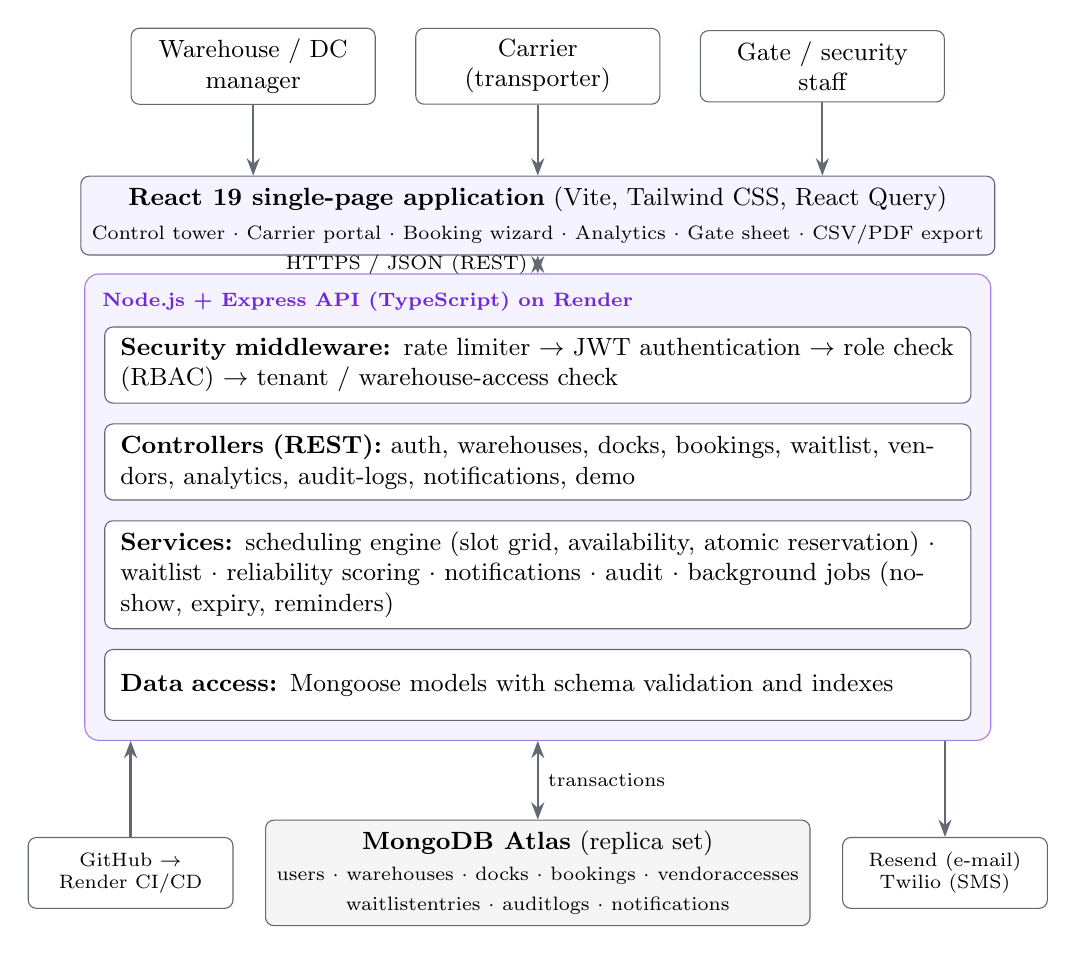
\begin{tikzpicture}[node distance=0.35cm and 0.3cm]
  % users
  \node[blk, minimum width=3.1cm] (u1) {Warehouse / DC\\manager};
  \node[blk, minimum width=3.1cm, right=0.5cm of u1] (u2) {Carrier\\(transporter)};
  \node[blk, minimum width=3.1cm, right=0.5cm of u2] (u3) {Gate / security\\staff};
  % presentation
  \node[blk, minimum width=11cm, below=0.9cm of u2, fill=boxbg] (spa) {\textbf{React 19 single-page application} (Vite, Tailwind CSS, React Query)\\[1pt]\scriptsize Control tower $\cdot$ Carrier portal $\cdot$ Booking wizard $\cdot$ Analytics $\cdot$ Gate sheet $\cdot$ CSV/PDF export};
  \draw[arr] (u1) -- (u1 |- spa.north);
  \draw[arr] (u2) -- (spa.north);
  \draw[arr] (u3) -- (u3 |- spa.north);
  % api
  \node[blk, minimum width=11cm, below=0.9cm of spa, align=left, text width=10.6cm] (mw) {\textbf{Security middleware:} rate limiter $\rightarrow$ JWT authentication $\rightarrow$ role check (RBAC) $\rightarrow$ tenant / warehouse-access check};
  \node[blk, minimum width=11cm, below=0.25cm of mw, align=left, text width=10.6cm] (ctl) {\textbf{Controllers (REST):} auth, warehouses, docks, bookings, waitlist, vendors, analytics, audit-logs, notifications, demo};
  \node[blk, minimum width=11cm, below=0.25cm of ctl, align=left, text width=10.6cm] (svc) {\textbf{Services:} scheduling engine (slot grid, availability, atomic reservation) $\cdot$ waitlist $\cdot$ reliability scoring $\cdot$ notifications $\cdot$ audit $\cdot$ background jobs (no-show, expiry, reminders)};
  \node[blk, minimum width=11cm, below=0.25cm of svc, align=left, text width=10.6cm] (mdl) {\textbf{Data access:} Mongoose models with schema validation and indexes};
  \begin{scope}[on background layer]
    \coordinate (apitop) at ($(mw.north)+(0,0.42)$);
    \node[layer, fit=(apitop)(mw)(ctl)(svc)(mdl), label={[lbl, anchor=north west, xshift=3pt, yshift=-3pt]north west:Node.js + Express API (TypeScript) on Render}] (api) {};
  \end{scope}
  \draw[darr] (spa.south) -- node[left, font=\scriptsize]{HTTPS / JSON (REST)} (api.north -| spa.south);
  % db
  \node[blk, minimum width=6cm, below=1.0cm of api, fill=gray!8] (db) {\textbf{MongoDB Atlas} (replica set)\\\scriptsize users $\cdot$ warehouses $\cdot$ docks $\cdot$ bookings $\cdot$ vendoraccesses\\\scriptsize waitlistentries $\cdot$ auditlogs $\cdot$ notifications};
  \draw[darr] (api.south -| db.north) -- node[right, font=\scriptsize]{transactions} (db.north);
  % external
  \node[blk, right=0.4cm of db, minimum width=2.6cm, font=\scriptsize] (ext) {Resend (e-mail)\\Twilio (SMS)};
  \draw[arr] (api.south -| ext.north) -- (ext.north);
  \node[blk, left=0.4cm of db, minimum width=2.6cm, font=\scriptsize] (ci) {GitHub $\rightarrow$\\Render CI/CD};
  \draw[arr] (ci.north) -- (api.south -| ci.north);
\end{tikzpicture}

\caption{System architecture of SmartDock}
\label{fig:arch}
\end{figure}

\section{Data Flow Diagrams}
Figure~\ref{fig:dfd0} shows the context (level-0) diagram: SmartDock exchanges information with three human actors and the notification providers. Figure~\ref{fig:dfd1} decomposes the system into six processes and five data stores.

\begin{figure}[!htbp]
\centering
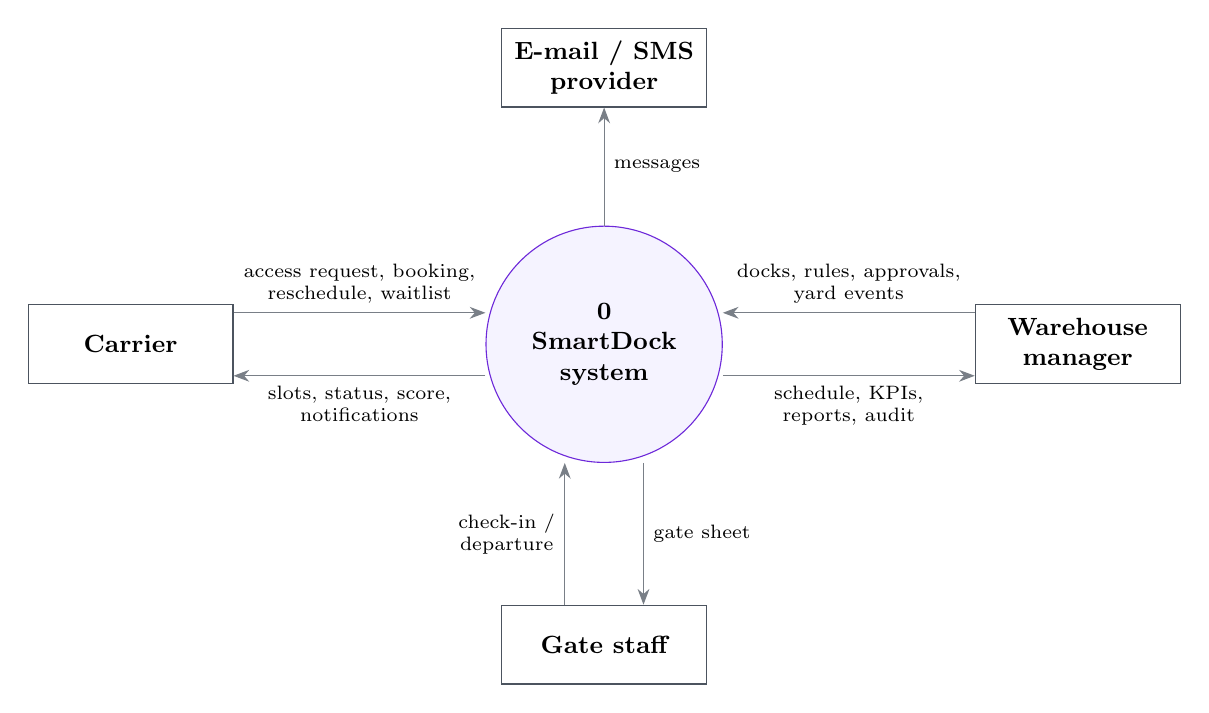
\begin{tikzpicture}
  \node[proc, minimum size=3cm, font=\small\bfseries] (sys) {0\\SmartDock\\system};
  \node[ent, left=3.2cm of sys] (car) {Carrier};
  \node[ent, right=3.2cm of sys] (mgr) {Warehouse\\manager};
  \node[ent, below=1.8cm of sys] (gate) {Gate staff};
  \node[ent, above=1.5cm of sys] (prov) {E-mail / SMS\\provider};
  \draw[flow] ([yshift=4mm]car.east) -- node[above]{access request, booking,\\reschedule, waitlist} ([yshift=4mm]sys.west);
  \draw[flow] ([yshift=-4mm]sys.west) -- node[below]{slots, status, score,\\notifications} ([yshift=-4mm]car.east);
  \draw[flow] ([yshift=4mm]mgr.west) -- node[above]{docks, rules, approvals,\\yard events} ([yshift=4mm]sys.east);
  \draw[flow] ([yshift=-4mm]sys.east) -- node[below]{schedule, KPIs,\\reports, audit} ([yshift=-4mm]mgr.west);
  \draw[flow] ([xshift=-5mm]gate.north) -- node[left]{check-in /\\departure} ([xshift=-5mm]sys.south);
  \draw[flow] ([xshift=5mm]sys.south) -- node[right]{gate sheet} ([xshift=5mm]gate.north);
  \draw[flow] (sys.north) -- node[right]{messages} (prov.south);
\end{tikzpicture}

\caption{Context diagram (DFD level 0)}
\label{fig:dfd0}
\end{figure}

\begin{figure}[!htbp]
\centering
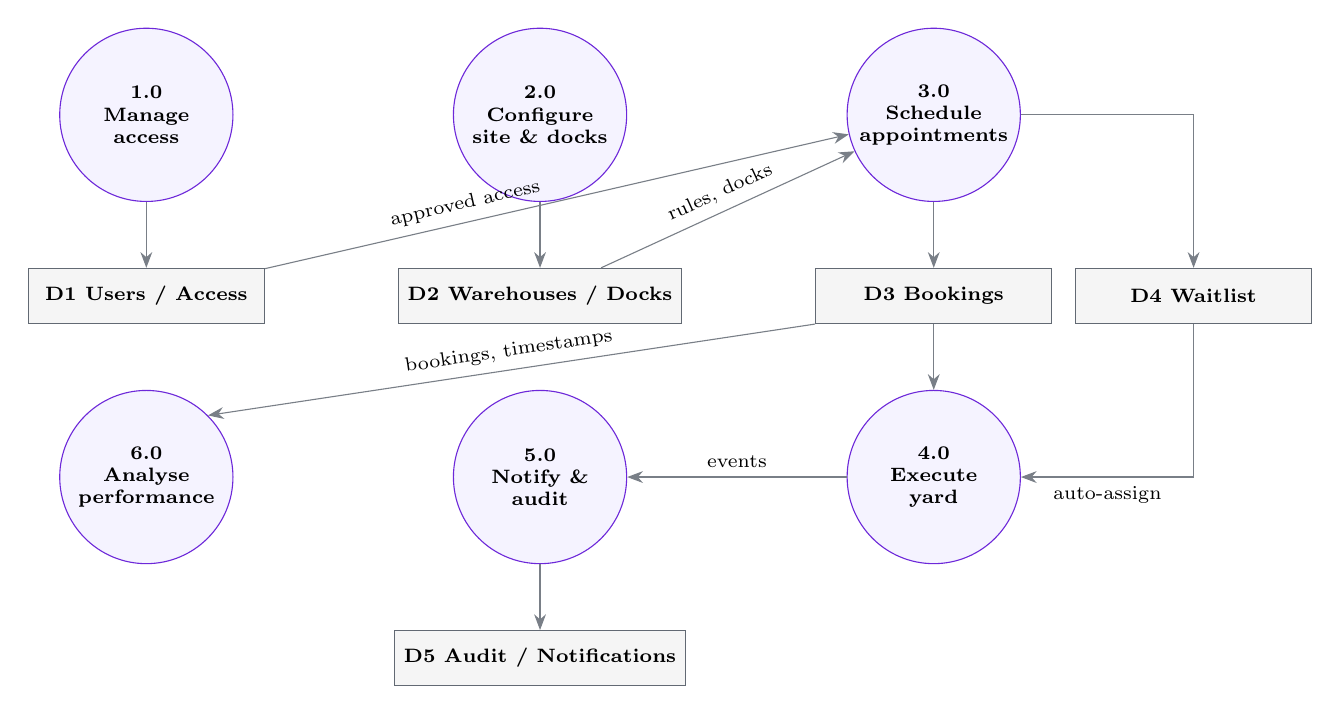
\begin{tikzpicture}[x=1cm,y=1cm]
  \node[proc] (p1) at (0,0) {1.0\\Manage\\access};
  \node[proc] (p2) at (5,0) {2.0\\Configure\\site \& docks};
  \node[proc] (p3) at (10,0) {3.0\\Schedule\\appointments};
  \node[proc] (p4) at (10,-4.6) {4.0\\Execute\\yard};
  \node[proc] (p5) at (5,-4.6) {5.0\\Notify \&\\audit};
  \node[proc] (p6) at (0,-4.6) {6.0\\Analyse\\performance};
  \node[store] (d1) at (0,-2.3) {D1 Users / Access};
  \node[store] (d2) at (5,-2.3) {D2 Warehouses / Docks};
  \node[store] (d3) at (10,-2.3) {D3 Bookings};
  \node[store] (d4) at (13.3,-2.3) {D4 Waitlist};
  \node[store] (d5) at (5,-6.9) {D5 Audit / Notifications};
  \draw[flow] (p1) -- (d1);
  \draw[flow] (p2) -- (d2);
  \draw[flow] (d2) -- node[above, sloped]{rules, docks} (p3);
  \draw[flow] (d1) -- node[above, sloped, pos=0.35]{approved access} (p3);
  \draw[flow] (p3) -- (d3);
  \draw[flow] (p3.east) -| (d4.north);
  \draw[flow] (d4.south) |- node[below, pos=0.75]{auto-assign} (p4.east);
  \draw[flow] (d3) -- (p4);
  \draw[flow] (p4) -- node[above]{events} (p5);
  \draw[flow] (p5) -- (d5);
  \draw[flow] (d3.south west) -- node[above, sloped]{bookings, timestamps} (p6.north east);
\end{tikzpicture}

\caption{Level-1 data flow diagram}
\label{fig:dfd1}
\end{figure}

\section{Use Case Diagram}
Figure~\ref{fig:usecase} shows what each actor can do. The scheduler represents the automated background jobs.

\begin{figure}[!htbp]
\centering
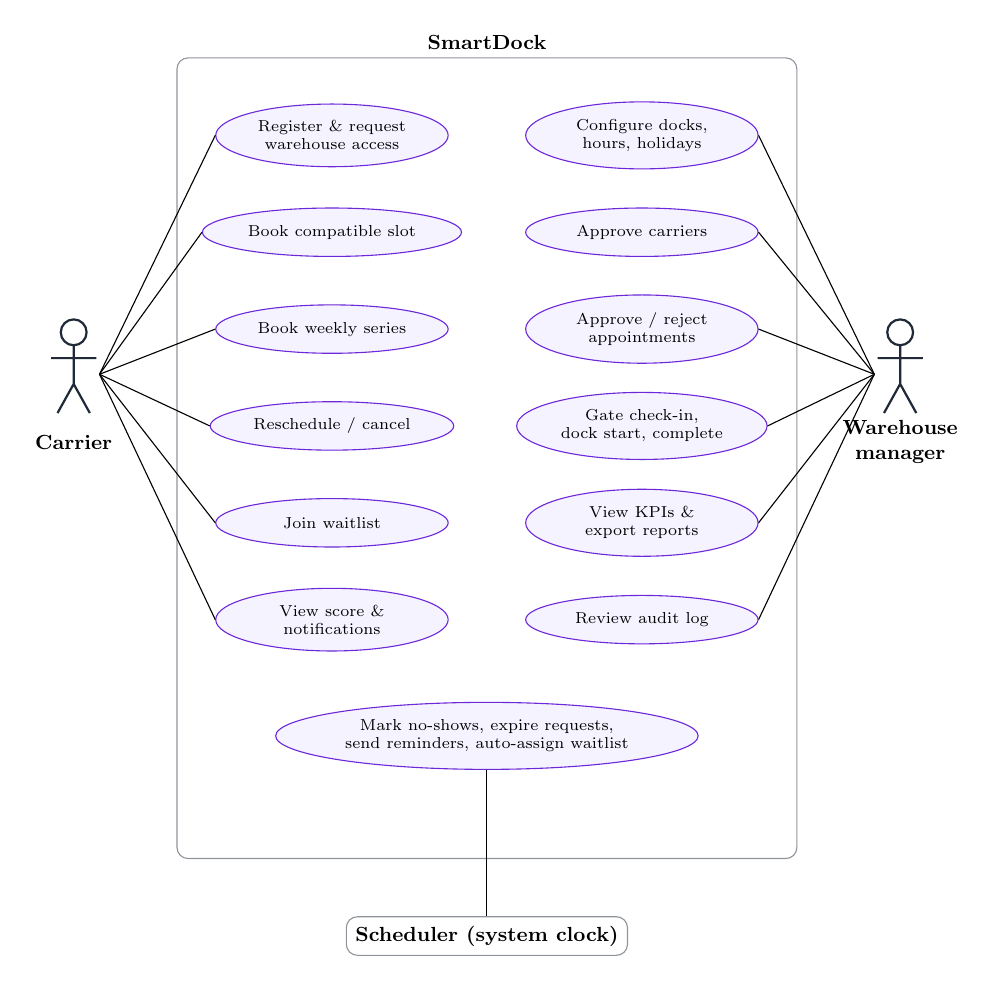
\begin{tikzpicture}[scale=0.82, transform shape, uc/.style={ellipse, draw=brand, fill=boxbg, font=\scriptsize, minimum width=3.6cm, minimum height=0.75cm, align=center},
  actor/.style={font=\small\bfseries, align=center}]
  \node[draw=ink!50, rounded corners, minimum width=9.6cm, minimum height=12.4cm, label={[font=\small\bfseries]north:SmartDock}] (box) at (0,0) {};
  % carrier use cases (left column)
  \node[uc] (c1) at (-2.4,5.0) {Register \& request\\warehouse access};
  \node[uc] (c2) at (-2.4,3.5) {Book compatible slot};
  \node[uc] (c3) at (-2.4,2.0) {Book weekly series};
  \node[uc] (c4) at (-2.4,0.5) {Reschedule / cancel};
  \node[uc] (c5) at (-2.4,-1.0) {Join waitlist};
  \node[uc] (c6) at (-2.4,-2.5) {View score \&\\notifications};
  % manager use cases (right column)
  \node[uc] (m1) at (2.4,5.0) {Configure docks,\\hours, holidays};
  \node[uc] (m2) at (2.4,3.5) {Approve carriers};
  \node[uc] (m3) at (2.4,2.0) {Approve / reject\\appointments};
  \node[uc] (m4) at (2.4,0.5) {Gate check-in,\\dock start, complete};
  \node[uc] (m5) at (2.4,-1.0) {View KPIs \&\\export reports};
  \node[uc] (m6) at (2.4,-2.5) {Review audit log};
  % system
  \node[uc] (s1) at (0,-4.3) {Mark no-shows, expire requests,\\send reminders, auto-assign waitlist};
  % stick-figure actors
  \foreach \x/\name in {-6.4/Carrier, 6.4/{Warehouse\\manager}} {
    \begin{scope}[shift={(\x,1.2)}]
      \draw[thick, ink] (0,0.75) circle (0.2);
      \draw[thick, ink] (0,0.55) -- (0,-0.05) (-0.35,0.35) -- (0.35,0.35) (0,-0.05) -- (-0.25,-0.5) (0,-0.05) -- (0.25,-0.5);
      \node[actor] at (0,-0.95) {\name};
    \end{scope}
  }
  \coordinate (car) at (-6.0,1.3);
  \coordinate (mgr) at (6.0,1.3);
  \node[actor, draw=ink!50, rounded corners, inner sep=4pt] (sys) at (0,-7.4) {Scheduler (system clock)};
  \foreach \u in {c1,c2,c3,c4,c5,c6} \draw (car.east) -- (\u.west);
  \foreach \u in {m1,m2,m3,m4,m5,m6} \draw (mgr.west) -- (\u.east);
  \draw (sys.north) -- (s1.south);
\end{tikzpicture}

\caption{Use case diagram}
\label{fig:usecase}
\end{figure}

\section{Entity--Relationship Diagram}
Figure~\ref{fig:er} shows the main collections and their relationships. MongoDB stores them as documents; references are ObjectIds and are enforced in application code.

\begin{figure}[!htbp]
\centering
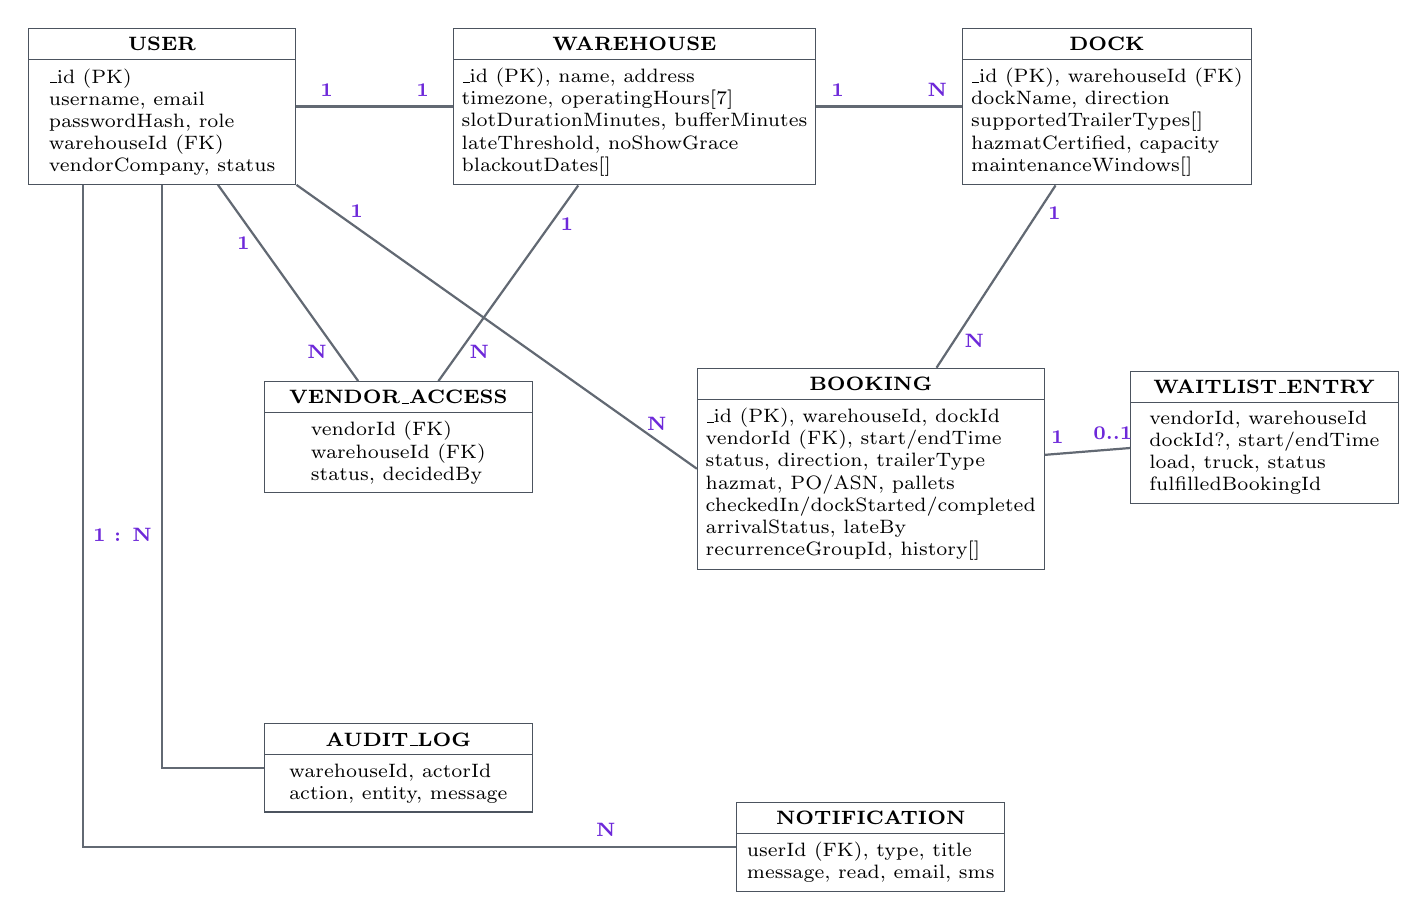
\begin{tikzpicture}[e/.style={rectangle split, rectangle split parts=2, draw=ink!80, fill=white, font=\scriptsize, align=left, rectangle split part fill={boxbg,white}, minimum width=3.4cm, inner sep=3pt},
  rel/.style={draw=ink!70, thick}, card/.style={font=\scriptsize\bfseries, color=brand}]
  \node[e] (user) at (0,0) {\textbf{USER}\nodepart{two}\_id (PK)\\username, email\\passwordHash, role\\warehouseId (FK)\\vendorCompany, status};
  \node[e] (wh) at (6,0) {\textbf{WAREHOUSE}\nodepart{two}\_id (PK), name, address\\timezone, operatingHours[7]\\slotDurationMinutes, bufferMinutes\\lateThreshold, noShowGrace\\blackoutDates[]};
  \node[e] (dock) at (12,0) {\textbf{DOCK}\nodepart{two}\_id (PK), warehouseId (FK)\\dockName, direction\\supportedTrailerTypes[]\\hazmatCertified, capacity\\maintenanceWindows[]};
  \node[e] (acc) at (3,-4.2) {\textbf{VENDOR\_ACCESS}\nodepart{two}vendorId (FK)\\warehouseId (FK)\\status, decidedBy};
  \node[e] (bk) at (9,-4.6) {\textbf{BOOKING}\nodepart{two}\_id (PK), warehouseId, dockId\\vendorId (FK), start/endTime\\status, direction, trailerType\\hazmat, PO/ASN, pallets\\checkedIn/dockStarted/completed\\arrivalStatus, lateBy\\recurrenceGroupId, history[]};
  \node[e] (wl) at (14,-4.2) {\textbf{WAITLIST\_ENTRY}\nodepart{two}vendorId, warehouseId\\dockId?, start/endTime\\load, truck, status\\fulfilledBookingId};
  \node[e] (au) at (3,-8.4) {\textbf{AUDIT\_LOG}\nodepart{two}warehouseId, actorId\\action, entity, message};
  \node[e] (nt) at (9,-9.4) {\textbf{NOTIFICATION}\nodepart{two}userId (FK), type, title\\message, read, email, sms};
  \draw[rel] (user) -- node[card, above]{1 \quad\quad\quad 1} (wh);
  \draw[rel] (wh) -- node[card, above]{1 \quad\quad\quad N} (dock);
  \draw[rel] (user) -- node[card, left, pos=0.3]{1}node[card, left, pos=0.85]{N} (acc);
  \draw[rel] (wh) -- node[card, right, pos=0.2]{1}node[card, right, pos=0.85]{N} (acc);
  \draw[rel] (dock) -- node[card, right, pos=0.15]{1}node[card, right, pos=0.85]{N} (bk);
  \draw[rel] (user.south east) -- node[card, above, pos=0.15]{1}node[card, above, pos=0.9]{N} (bk.west);
  \draw[rel] (wl) -- node[card, above, pos=0.2]{0..1}node[card, above, pos=0.85]{1} (bk);
  \draw[rel] (user.south) |- node[card, left, pos=0.3]{1 : N} (au.west);
  \draw[rel] (user.south) ++(-1,0) |- node[card, pos=0.9, above]{N} (nt.west);
\end{tikzpicture}

\caption{Entity--relationship diagram}
\label{fig:er}
\end{figure}

\section{Appointment Lifecycle}
Each booking follows a finite-state machine (Figure~\ref{fig:states}). Terminal states can never be revived, so capacity released by a cancellation cannot be silently re-occupied.

\begin{figure}[!htbp]
\centering
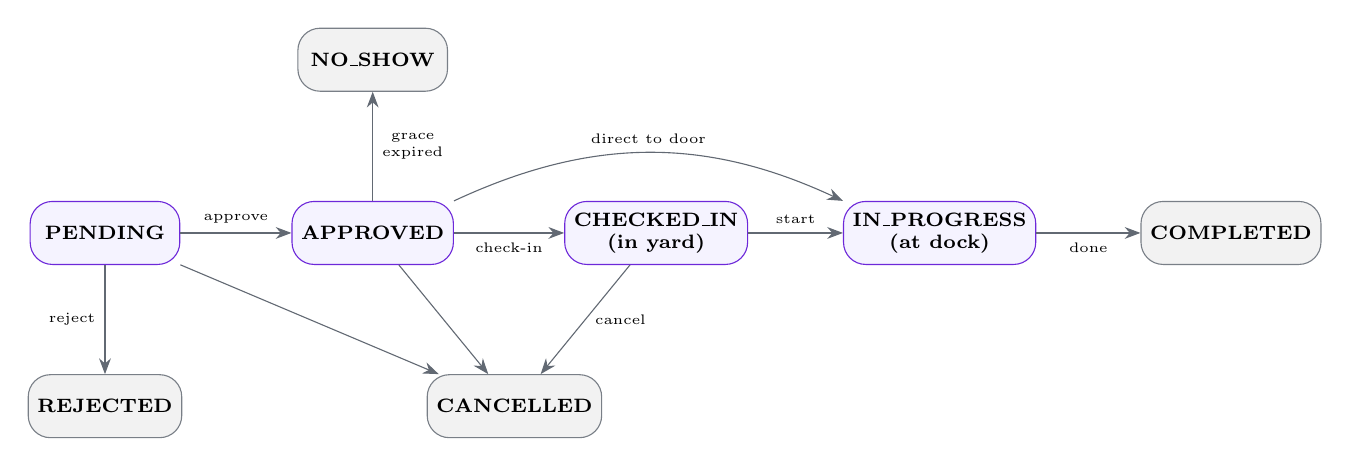
\begin{tikzpicture}[st/.style={rounded corners=8pt, draw=brand, fill=boxbg, font=\scriptsize\bfseries, minimum width=1.9cm, minimum height=0.8cm, align=center},
  term/.style={st, draw=ink!60, fill=gray!10}, t/.style={-{Stealth[length=2mm]}, draw=ink!70, font=\tiny, align=center}]
  \node[st] (p) at (0,0) {PENDING};
  \node[st] (a) at (3.4,0) {APPROVED};
  \node[st] (c) at (7.0,0) {CHECKED\_IN\\(in yard)};
  \node[st] (i) at (10.6,0) {IN\_PROGRESS\\(at dock)};
  \node[term] (d) at (14.3,0) {COMPLETED};
  \node[term] (r) at (0,-2.2) {REJECTED};
  \node[term] (x) at (5.2,-2.2) {CANCELLED};
  \node[term] (n) at (3.4,2.2) {NO\_SHOW};
  \draw[t] (p) -- node[above]{approve} (a);
  \draw[t] (a) -- node[below]{check-in} (c);
  \draw[t] (c) -- node[above]{start} (i);
  \draw[t] (i) -- node[below]{done} (d);
  \draw[t] (a.north east) to[bend left=25] node[above]{direct to door} (i.north west);
  \draw[t] (p) -- node[left]{reject} (r);
  \draw[t] (p) -- (x);
  \draw[t] (a) -- (x);
  \draw[t] (c) -- node[right]{cancel} (x);
  \draw[t] (a) -- node[right]{grace\\expired} (n);
\end{tikzpicture}

\caption{Booking state machine}
\label{fig:states}
\end{figure}

\section{Technology Stack}
\begin{table}[H]
\centering
\small
\caption{Technology stack}
\label{tab:stack}
\begin{tabularx}{\textwidth}{>{\bfseries\raggedright\arraybackslash}p{3.0cm}X}
\toprule
Layer & Technologies and purpose \\
\midrule
Language & TypeScript (strict mode) on both client and server \\
Frontend & React 19 \cite{react}, Vite 8, Tailwind CSS 4, TanStack React Query (data fetching, polling), React Router, React Hook Form + Zod (forms), date-fns, jsPDF + AutoTable (PDF export) \\
Backend & Node.js 22, Express 4 \cite{express}, Zod (request validation), JSON Web Tokens, bcrypt password hashing, express-rate-limit, Winston logging \\
Database & MongoDB Atlas (managed replica set) with Mongoose 8 ODM; multi-document transactions, compound indexes, aggregation pipelines \\
APIs & REST/JSON API (about 40 endpoints); Resend e-mail API and Twilio SMS API (optional) \\
Cloud \& DevOps & Render web service \cite{render} (Blueprint \texttt{render.yaml}, auto-deploy from GitHub), MongoDB Atlas free tier, GitHub for version control \\
Testing & End-to-end verification script with \texttt{mongodb-memory-server} (in-memory replica set) and two concurrent API instances; tenant-isolation unit test \\
Tools & Visual Studio Code, Git, npm, oxlint, Python + matplotlib (analysis and simulation), \LaTeX{} (this report) \\
\bottomrule
\end{tabularx}
\end{table}

\chapter{Modules Description}
SmartDock is organised into ten functional modules. Table~\ref{tab:modules} summarises them; the sections that follow describe each in supply-chain terms.

\begin{table}[H]
\centering
\small
\caption{Functional modules and their main users}
\label{tab:modules}
\begin{tabularx}{\textwidth}{>{\raggedright\arraybackslash}p{4.2cm}X>{\raggedright\arraybackslash}p{2.4cm}}
\toprule
\textbf{Module} & \textbf{Responsibility} & \textbf{Used by} \\
\midrule
1. Identity \& access & Registration, login, roles, per-warehouse carrier approval & All \\
2. Site \& dock configuration & Docks, equipment, capacity, hours, slot rules, holidays, maintenance & Manager \\
3. Scheduling engine & Slot grid, availability, load--dock matching, atomic reservation & System \\
4. Appointment booking & Booking wizard, recurring series, rescheduling, cancellation & Carrier, manager \\
5. Waitlist & Queue for full slots, automatic FIFO assignment & Carrier, system \\
6. Yard execution & Approvals, gate check-in, dock start, completion, no-shows & Manager, gate \\
7. Carrier performance & Punctuality tracking, reliability score and tier & Manager, carrier \\
8. Analytics \& reporting & KPIs, charts, heatmap, CSV/PDF export, gate sheet & Manager \\
9. Notifications & In-app centre, e-mail, SMS, reminders & All \\
10. Audit trail & Persistent, filterable log of every action & Manager \\
\bottomrule
\end{tabularx}
\end{table}

\section{Identity and Access Management}
Three roles exist: \textbf{warehouse manager}, \textbf{carrier} and \textbf{super administrator}. A manager registers together with the warehouse they run. A carrier registers with its company name and selects the warehouses it wants to serve; each selection creates a \emph{vendor-access request}. A warehouse's manager sees only requests for that warehouse and can approve, reject or later revoke them. A carrier can see availability and book \emph{only} at warehouses that approved it, and the check is repeated on every request so a revocation takes effect immediately. Super administrators cannot be created through the public sign-up form; they are created on the server with a command-line script. Passwords are stored as bcrypt hashes and sessions use signed JSON Web Tokens.

\section{Site and Dock Configuration}
The manager models the physical facility:
\begin{itemize}
  \item \textbf{Dock doors} --- name, movement direction (inbound, outbound or both), supported trailer types (dry van, reefer, flatbed, container), hazmat certification and capacity (trucks per slot).
  \item \textbf{Operating hours} --- per weekday, with an open/closed flag.
  \item \textbf{Appointment rules} --- slot length (15, 30, 60 or 90 minutes), turnover buffer between consecutive slots, late-arrival threshold and no-show grace period.
  \item \textbf{Blackout dates} --- public holidays, stock-takes and shutdowns on which the site is closed.
  \item \textbf{Maintenance windows} --- planned downtime of a single door; the system lists the existing appointments that overlap so they can be moved.
\end{itemize}

\section{Scheduling Engine}
The engine converts the rules into concrete, bookable slots for any date, in the warehouse's own time zone. For each active dock that is compatible with the requested load it reports, per slot, the remaining capacity and the reason a slot is unavailable (\emph{full}, \emph{maintenance} or \emph{past}). It also validates every booking request against the same grid and performs the atomic capacity reservation described in Chapter~\ref{ch:impl}.

\section{Appointment Booking}
Carriers book through a four-step wizard: (1) site and load details --- inbound or outbound, trailer type, hazmat; (2) date and slot, showing only compatible docks; (3) shipment details --- truck number, driver name and mobile, PO/ASN reference, pallet count, cargo; (4) confirmation. A booking may be made as a \textbf{weekly recurring series} of 2--12 weeks; each week is reserved independently and weeks that are closed or full are reported back rather than failing the whole series. Carriers and managers can \textbf{reschedule} an appointment to another slot or door; the history of moves is stored, and a carrier's move of a confirmed appointment returns it to the manager for re-approval. An entire series can be cancelled in one action.

\section{Waitlist}
If the desired slot is full, the carrier can join its \textbf{waitlist}, for a specific door or for any compatible door. Whenever capacity is released --- by a cancellation, a rejection or a reschedule --- the system automatically converts the oldest compatible waiting entry into a booking (first-in, first-out), marks the entry as fulfilled and notifies both sides. Entries whose slot has passed expire automatically.

\section{Yard Execution}
The \emph{Yard schedule} screen is the manager's daily control tower. For the selected day it lists every truck with its door, carrier, driver, load and references, and offers the next valid action: \emph{Approve/Reject} for requests, \emph{Gate check-in} when the truck arrives, \emph{Start at dock} when loading begins, and \emph{Complete \& depart}. The system timestamps each event, classifies the arrival as \emph{on time} or \emph{late} against the warehouse threshold, and records the delay in minutes. Confirmed trucks that do not arrive within the grace period are marked \emph{no-show} automatically; requests that were never approved expire when their slot starts. A printable \emph{gate sheet} gives security staff the day's expected trucks with columns for gate times, seal numbers and signatures.

\section{Carrier Performance}
Every arrival and no-show feeds the carrier's \textbf{reliability score}:
\begin{equation}
\text{Reliability} = \frac{\text{on-time arrivals} + 0.5\times\text{late arrivals}}{\text{arrivals} + \text{no-shows}}\times 100
\end{equation}
Scores map to tiers: \textbf{A} ($\geq 90$, excellent), \textbf{B} ($\geq 75$, good), \textbf{C} ($\geq 50$, needs improvement) and \textbf{D} (below 50, poor). Managers see the score and tier when approving a new carrier and in a scorecard table; carriers see their own score on their dashboard, which creates an incentive to arrive on time.

\section{Analytics and Reporting}
For any date range, the analytics module reports: total appointments and daily average; \textbf{dock utilisation} (booked truck-slots divided by offered truck-slots, excluding closures and maintenance); on-time, no-show and cancellation rates; average \textbf{turnaround}, \textbf{yard wait} and \textbf{dock time}; pallets handled; a daily volume chart; a weekday $\times$ hour \textbf{demand heatmap}; the busiest hours; utilisation per door; the inbound/outbound and equipment mix; and a carrier performance table. Results can be exported as CSV or as a formatted PDF KPI report.

\section{Notifications}
Each event creates an in-app notification for the relevant party (shown under a bell icon with an unread counter), for example: new request, approval, rejection, rescheduling, cancellation, waitlist assignment, no-show and new carrier access request. About 24 hours before a confirmed appointment a reminder is sent to the carrier and, when SMS is configured, to the driver's mobile. E-mail (Resend) and SMS (Twilio) are activated simply by adding API keys; delivery status is stored with each notification.

\section{Audit Trail}
Every change --- bookings and status changes, reschedules, waitlist events, dock and rule changes, holidays, maintenance and carrier-access decisions --- is written to an audit collection with the actor, role, time, action and a human-readable message. Automated actions are attributed to ``SmartDock automation''. Managers can filter, search, page through and export the log for their own warehouse only, which supports dispute resolution (for example, detention claims) and compliance.

\chapter{Implementation Details}\label{ch:impl}
This chapter explains the key algorithms. Complete source code is available in the GitHub repository; the most important excerpts are reproduced in Appendix~\ref{app:code}.

\section{Project Structure}
\begin{itemize}
  \item \texttt{client/} --- React application: \texttt{pages/admin} (control-tower tabs and gate sheet), \texttt{pages/vendor} (carrier portal and booking wizard), \texttt{components} (slot picker, reschedule dialog, notification bell, UI kit), \texttt{lib} (formatting and CSV/PDF export).
  \item \texttt{server/src/models} --- Mongoose schemas: User, Warehouse, Dock, Booking, VendorAccess, WaitlistEntry, AuditLog, Notification.
  \item \texttt{server/src/services} --- business logic: \texttt{scheduling}, \texttt{waitlist}, \texttt{reliability}, \texttt{notifications}, \texttt{audit}, \texttt{jobs}, \texttt{seed}.
  \item \texttt{server/src/controllers} and \texttt{routes} --- the REST API; \texttt{middleware} --- authentication, roles and tenant access.
  \item \texttt{render.yaml} --- infrastructure-as-code definition of the cloud deployment.
\end{itemize}

\section{Time-Zone-Correct Slot Generation}
Warehouses operate in local time, but all instants are stored in UTC so that sites in different zones and daylight-saving transitions are handled correctly. Given a local date $d$, the engine:
\begin{enumerate}
  \item returns \emph{closed} if $d$ is a blackout date or the weekday is closed;
  \item converts opening time $o$ and closing time $c$ to minutes and generates slots
  \[ s_k = o + k\,(L + B), \qquad e_k = s_k + L, \qquad \text{while } e_k \le c, \]
  where $L$ is the slot length and $B$ the turnover buffer (e.g.\ $L=30$, $B=15$ gives 08:00--08:30, 08:45--09:15, \ldots);
  \item converts each local start and end to an exact UTC instant using the IANA time-zone database. Because a local time's UTC offset depends on the date, the conversion starts from a guess and corrects it by the observed difference until it converges (at most three iterations; Listing~\ref{lst:tz}).
\end{enumerate}
For availability, each slot of each compatible door is then checked against existing active bookings (overlap test $a_s < b_e \wedge a_e > b_s$), maintenance windows and the current time.

\section{Load--Dock Compatibility}
A load is described by its direction, trailer type and hazmat flag. A dock is compatible if (i) its direction is \emph{both} or equals the load's direction, (ii) its supported trailer types include the load's type, and (iii) it is hazmat-certified whenever the load is hazardous. Incompatible doors are never shown to the carrier, and the same rule is re-checked on the server when a booking is submitted (Listing~\ref{lst:compat}).

\section{Atomic Capacity Reservation}
The central correctness requirement is that a slot with capacity $C$ never holds more than $C$ active bookings. A naive implementation ``count overlapping bookings, then insert if fewer than $C$'' is unsafe: two requests can both count $C-1$ and both insert --- the \emph{write-skew} anomaly \cite{kleppmann2017}. Running both steps inside a database transaction is \emph{not} sufficient by itself, because each transaction reads its own snapshot and they write different documents, so the database sees no conflict.

SmartDock therefore uses two layers (Listing~\ref{lst:reserve}):
\begin{enumerate}
  \item \textbf{In-process lock per dock.} Requests for the same door handled by one server process are queued and executed one at a time.
  \item \textbf{Dock write lock inside a MongoDB transaction.} Each reservation transaction first increments a counter field on the \emph{dock document}, then counts overlapping active bookings and inserts only if the count is below capacity. Because every concurrent reservation for the same door now writes the same document, MongoDB detects a write conflict, aborts all but one transaction and the driver retries them; the retries see the committed booking and are rejected with HTTP 409 if the slot is full. This holds across any number of server instances.
\end{enumerate}
The same routine is reused for new bookings, each week of a recurring series, rescheduling (excluding the booking being moved) and waitlist assignment. If transactions are unavailable (a standalone development database), the system falls back to the in-process lock and logs a warning.

\begin{figure}[H]
\centering
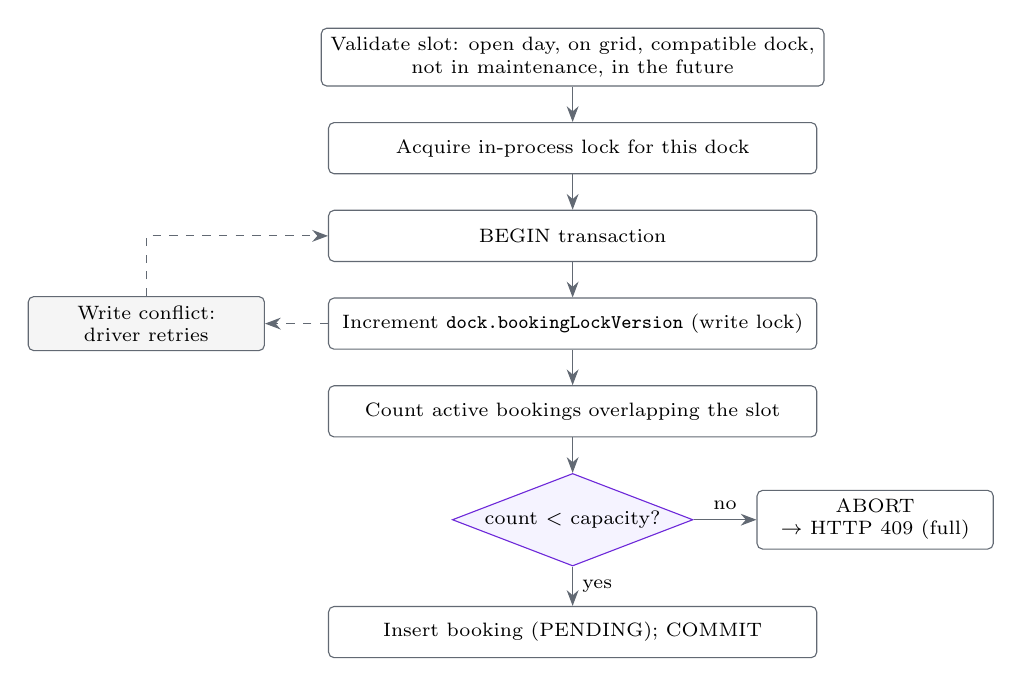
\begin{tikzpicture}[node distance=0.45cm, every node/.style={font=\scriptsize}]
  \tikzset{fb/.style={draw=ink!70, rounded corners=2pt, fill=white, align=center, minimum width=6.2cm, minimum height=0.65cm},
           fd/.style={diamond, aspect=2.6, draw=brand, fill=boxbg, align=center, inner sep=1pt},
           fa/.style={-{Stealth[length=2mm]}, draw=ink!70}}
  \node[fb] (a) {Validate slot: open day, on grid, compatible dock,\\not in maintenance, in the future};
  \node[fb, below=of a] (b) {Acquire in-process lock for this dock};
  \node[fb, below=of b] (c) {BEGIN transaction};
  \node[fb, below=of c] (d) {Increment \texttt{dock.bookingLockVersion} (write lock)};
  \node[fb, below=of d] (e) {Count active bookings overlapping the slot};
  \node[fd, below=of e] (f) {count $<$ capacity?};
  \node[fb, below=0.5cm of f] (g) {Insert booking (PENDING); COMMIT};
  \node[fb, right=0.8cm of f, minimum width=3.0cm] (h) {ABORT\\$\rightarrow$ HTTP 409 (full)};
  \node[fb, left=0.8cm of d, minimum width=3.0cm, fill=gray!8] (r) {Write conflict:\\driver retries};
  \draw[fa] (a) -- (b); \draw[fa] (b) -- (c); \draw[fa] (c) -- (d); \draw[fa] (d) -- (e); \draw[fa] (e) -- (f);
  \draw[fa] (f) -- node[right]{yes} (g); \draw[fa] (f) -- node[above]{no} (h);
  \draw[fa, dashed] (d.west) -- (r.east); \draw[fa, dashed] (r.north) |- (c.west);
\end{tikzpicture}

\caption{Atomic capacity reservation algorithm}
\label{fig:reserve}
\end{figure}

\section{Recurring Bookings and Rescheduling}
For a weekly series of $n$ weeks, the local start time of the first slot (e.g.\ 09:00) is kept and, for each week $k$, the slot with the same local start on date $d+7k$ is looked up in that day's grid. This keeps the appointment at 09:00 local time even across daylight-saving changes. Each week is validated and reserved separately; failures are collected as ``skipped weeks''. Rescheduling validates the new slot with the same rules, reserves capacity while excluding the booking itself, records the move in the booking's history and finally offers the released old slot to the waitlist.

\section{Waitlist Auto-Assignment}
When capacity is released on a door and slot, the waitlist service selects \texttt{WAITING} entries for exactly that slot (for that door or ``any door''), ordered by creation time. For each entry it re-checks dock compatibility and the carrier's access, then calls the reservation routine. Inside the same transaction it marks the entry \texttt{FULFILLED}, so an entry can never be assigned twice. The loop stops at the first ``slot full'' result (Listing~\ref{lst:waitlist}).

\section{Arrival Classification and Background Jobs}
At gate check-in the delay is computed as $\Delta = t_\text{check-in} - t_\text{slot start}$ in minutes; the arrival is \emph{late} if $\Delta$ exceeds the warehouse's threshold (default 15 minutes) and \emph{on time} otherwise, including early arrivals. A background job runs every minute and (i) marks confirmed bookings as \texttt{NO\_SHOW} when the grace period after the slot start has elapsed without check-in, (ii) expires pending requests whose slot has started, (iii) sends reminders for confirmed appointments in the next 24 hours, and (iv) expires waitlist entries for past slots. Every update is conditional on the previous state, so the job is safe to run on several instances at once (Listing~\ref{lst:jobs}).

\section{Security Measures}
\begin{itemize}
  \item \textbf{Authentication}: bcrypt-hashed passwords, signed JWTs with expiry; the client stores the session and logs out automatically on token expiry.
  \item \textbf{Authorisation}: role checks on every route and a \emph{tenant} check that pins managers to their own warehouse and carriers to warehouses that approved them (Listing~\ref{lst:access}); identifiers are taken from the verified token, never trusted from the request body. This addresses broken access control, the top risk in the OWASP Top 10 \cite{owasp2021}.
  \item \textbf{Validation}: every request body is validated with Zod schemas; database schemas validate again before writing.
  \item \textbf{Abuse protection}: rate limiting on the API; super administrators cannot self-register.
\end{itemize}

\section{Deployment}
The Express server serves both the API and the compiled React files, so the system is a single Render web service. The \texttt{render.yaml} Blueprint declares the build command (build client, then server), start command, health check, auto-deploy on every push to the \texttt{main} branch and the environment variables (database URI, generated JWT secret, optional e-mail/SMS keys and demo mode). The database is a MongoDB Atlas free-tier replica set in the Mumbai region. In demo mode the server seeds realistic data on first start and offers a ``Reset demo data'' action.

\chapter{Screenshots and Live Demo}
The system is live at \url{\LiveURL}. The screenshots below were captured from the running application with the demo dataset (Chennai Central Distribution Centre, five dock doors, six carriers). Demo logins: \texttt{admin@smartdock.demo} (warehouse manager) and \texttt{carrier@smartdock.demo} (carrier), password \texttt{Demo@123}.

\newcommand{\shotpair}[6]{% fileA, captionA, fileB, captionB, label, main caption
  \begin{figure}[H]\centering
  \begin{subfigure}[t]{0.49\textwidth}\centering\fbox{\includegraphics[width=0.96\textwidth]{#1}}\caption{#2}\end{subfigure}\hfill
  \begin{subfigure}[t]{0.49\textwidth}\centering\fbox{\includegraphics[width=0.96\textwidth]{#3}}\caption{#4}\end{subfigure}
  \caption{#6}\label{#5}\end{figure}}

\noindent\textbf{Warehouse manager (control tower).} Figures~\ref{fig:s-login}--\ref{fig:s-gate}.
\shotpair{login.jpg}{Login with one-click demo accounts}{admin_calendar.jpg}{Control tower and appointment calendar}{fig:s-login}{Entry point and manager overview}
\begin{figure}[H]\centering
\fbox{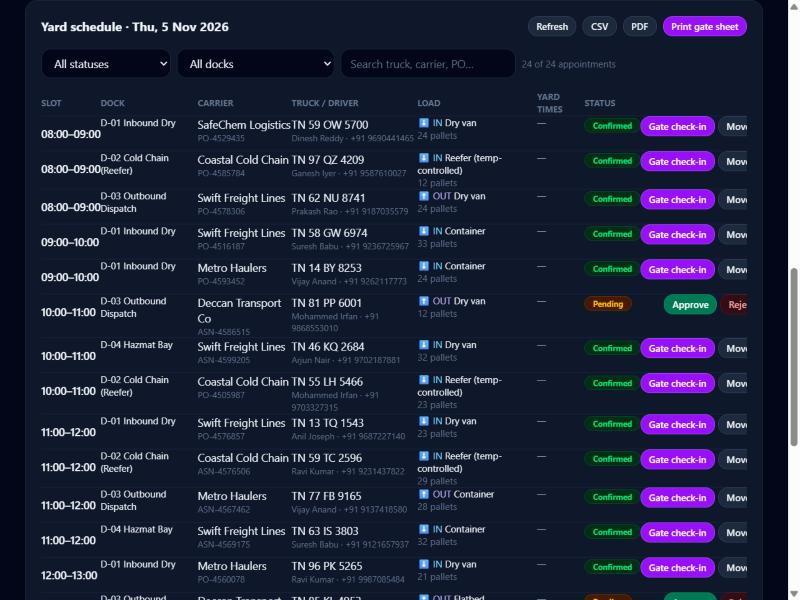
\includegraphics[width=0.72\textwidth]{yard_schedule.jpg}}
\caption{Yard schedule: door, carrier, PO/ASN, truck, driver, load and the next action for each truck}\label{fig:s-yard}
\end{figure}
\shotpair{docks.jpg}{Dock doors: direction, trailer types, hazmat, capacity and a maintenance window}{carriers.jpg}{Carrier access request and scorecard with reliability tiers}{fig:s-docks}{Dock configuration and carrier management}
\shotpair{analytics_kpis.jpg}{KPI cards, daily volume and busiest hours}{analytics_heatmap.jpg}{Demand heatmap, utilisation per door and load mix}{fig:s-heat}{Analytics and KPIs}
\shotpair{settings.jpg}{Scheduling rules with live slot preview, hours and holidays}{activity_log.jpg}{Activity log: holiday, waitlist auto-assignment, cancellation, check-in, rejection}{fig:s-audit}{Scheduling rules and audit trail}
\shotpair{notifications.jpg}{Notification centre}{gate_sheet.jpg}{Printable daily gate sheet for security staff}{fig:s-gate}{Notifications and gate operations}

\noindent\textbf{Carrier portal and booking wizard.} Figures~\ref{fig:s-carrier}--\ref{fig:s-b5}.
\shotpair{carrier_dashboard.jpg}{Carrier dashboard: reliability score, access status, appointments}{booking_step1.jpg}{Step 1: site, movement, trailer type, hazmat}{fig:s-carrier}{Carrier dashboard and booking wizard (1)}
\shotpair{booking_slots.jpg}{Step 2: only the reefer dock is offered; full slots offer the waitlist}{booking_details.jpg}{Step 3: truck, driver, PO/ASN, pallets and weekly recurrence}{fig:s-b2}{Booking wizard (2): slot selection and shipment details}
\shotpair{booking_confirm.jpg}{Step 4: confirmation summary}{booking_result.jpg}{Result: 3 of 4 weekly appointments booked, one full week skipped}{fig:s-b5}{Booking wizard (3): confirmation and weekly-series result}

\chapter{Testing and Validation}

\section{Testing Strategy}
\begin{itemize}
  \item \textbf{Static checks:} TypeScript strict type-checking of client and server on every build; \texttt{oxlint} for the client.
  \item \textbf{Unit test:} tenant isolation of dock updates, run against a mocked database.
  \item \textbf{End-to-end test suite} (\texttt{npm run verify:critical}): starts a throw-away in-memory MongoDB \emph{replica set} and \textbf{two} independent API server processes, then drives the real HTTP API through 58 checks covering security, concurrency, scheduling rules and business workflows. Running two servers makes the concurrency test meaningful for a multi-instance cloud deployment.
  \item \textbf{Manual UI testing:} every screen was exercised in the browser with the demo data (Chapter~6).
  \item \textbf{Live smoke test:} after deployment, logins, analytics, booking, approval, gate check-in, cancellation and the audit log were verified against the production URL and database.
\end{itemize}

\section{Test Cases}
Table~\ref{tab:tests} lists representative test cases from the 58 automated checks. All passed.

{\small
\begin{longtable}{>{\raggedright\arraybackslash}p{0.7cm}>{\raggedright\arraybackslash}p{6.2cm}>{\raggedright\arraybackslash}p{5.6cm}c}
\caption{Representative automated test cases}\label{tab:tests}\\
\toprule
\textbf{ID} & \textbf{Test case} & \textbf{Expected result} & \textbf{Status}\\
\midrule
\endfirsthead
\toprule
\textbf{ID} & \textbf{Test case} & \textbf{Expected result} & \textbf{Status}\\
\midrule
\endhead
\multicolumn{4}{l}{\textit{Security and multi-tenancy}}\\
T01 & Register a SUPER\_ADMIN through the public API & Rejected (400) & Pass\\
T02 & Unapproved carrier requests slot availability & Forbidden (403) & Pass\\
T03 & Manager of warehouse B lists or approves a request for warehouse A & Not visible; approval returns 404 & Pass\\
T04 & Carrier approved at A tries to book at B & Forbidden (403) & Pass\\
T05 & Manager B changes a booking of warehouse A & Forbidden (403) & Pass\\
T06 & Manager A reads warehouse B's audit log & B's events not returned & Pass\\
\multicolumn{4}{l}{\textit{Capacity and concurrency}}\\
T07 & 40 simultaneous bookings, capacity-1 slot, two servers & Exactly 1 created, 39 rejected (409) & Pass\\
T08 & 40 simultaneous bookings, capacity-3 slot, two servers & Exactly 3 created, 37 rejected (409) & Pass\\
T09 & Availability after T08 & Slot shows 0 remaining & Pass\\
T10 & Bookings use database transactions & No fallback warning logged & Pass\\
\multicolumn{4}{l}{\textit{Scheduling rules}}\\
T11 & Booking not aligned to the slot grid (09:15) & Rejected (400) & Pass\\
T12 & Booking outside operating hours (03:00) & Rejected (400) & Pass\\
T13 & Set 30-min slots + 15-min buffer & Grid 08:00--08:30, 08:45--09:15, \ldots & Pass\\
T14 & Unsupported slot length (45 min) & Rejected (400) & Pass\\
T15 & Reefer load requests availability & Only the reefer dock is listed & Pass\\
T16 & Dry-van truck books the reefer-only dock & Rejected (400) & Pass\\
T17 & Booking during a maintenance window & Slot marked MAINTENANCE; booking rejected & Pass\\
T18 & Booking on a blackout date & Day closed with reason; booking rejected & Pass\\
\multicolumn{4}{l}{\textit{Lifecycle and workflows}}\\
T19 & COMPLETED $\rightarrow$ PENDING; CANCELLED $\rightarrow$ APPROVED & Both rejected (400) & Pass\\
T20 & Carrier cancels a truck already at the dock & Rejected (400) & Pass\\
T21 & Mark no-show before the slot starts & Rejected (400) & Pass\\
T22 & Weekly series of 3 weeks & 3 appointments created & Pass\\
T23 & Join waitlist for a slot that still has space & Rejected (409) & Pass\\
T24 & Cancel a booking with a carrier waiting & Waitlisted carrier auto-booked; entry FULFILLED; notified & Pass\\
T25 & Reschedule to a free slot / to a full slot & 200 with history / 409 & Pass\\
T26 & Gate check-in, dock start, complete & Timestamps stored; arrival ON\_TIME & Pass\\
T27 & Reliability after one on-time trip & Score 100, tier A & Pass\\
T28 & Cancel remaining weekly series & 2 remaining appointments cancelled & Pass\\
T29 & Audit log after the workflow & All action types recorded & Pass\\
T30 & Analytics for the period & KPIs, per-dock utilisation and 7$\times$24 heatmap returned & Pass\\
\bottomrule
\end{longtable}
}

\section{Concurrency Experiment}\label{sec:concurrency}
To verify that test T07 is meaningful, the same test was run with both protection layers temporarily disabled. In that case the reservation logic behaves like a naive ``check then insert'' inside a transaction.

\begin{table}[H]
\centering
\caption{Double-booking experiment: 40 simultaneous requests across two servers}
\label{tab:conc}
\small
\begin{tabular}{>{\raggedright\arraybackslash}p{5.4cm}cc}
\toprule
\textbf{Configuration} & \textbf{Capacity-1 slot} & \textbf{Capacity-3 slot}\\
\midrule
Naive check-then-insert (protections disabled) & 15 (\textbf{14 over}) & 13 (\textbf{10 over}) \\
SmartDock reservation algorithm & \textbf{1} & \textbf{3} \\
\bottomrule
\end{tabular}
\end{table}

\section{Performance}
Response times were measured from a client in India against the live deployment (Render free tier, Oregon region; MongoDB Atlas M0, Mumbai region), 15 sequential requests per endpoint after a warm-up request. The health check, which does no database work, represents the network round-trip time.

\begin{table}[H]
\centering
\caption{Live API response times}
\label{tab:perf}
\begin{tabular}{lrr}
\toprule
\textbf{Endpoint} & \textbf{Median} & \textbf{90th percentile}\\
\midrule
Health check & 666 ms & 757 ms\\
Slot availability (1 day) & 1,338 ms & 1,433 ms\\
Yard schedule (1 day) & 1,575 ms & 1,904 ms\\
Analytics (30 days) & 4,300 ms & 6,719 ms\\
\bottomrule
\end{tabular}
\end{table}

During testing the analytics endpoint initially took about 5.8~s (median). Profiling showed that a new time-zone formatter object was created for every slot conversion; caching these objects reduced the median to the value above. The remaining latency is dominated by geography rather than computation: the free web service runs in Render's Oregon (USA) region while the database is in Mumbai, so every database query crosses the Pacific (roughly 0.2--0.3~s per round trip), and the health check alone shows a 0.5--0.7~s round trip from India to the server. The analytics request also transfers about 900 appointment documents. Moving the web service to an Asian region (e.g.\ Render Singapore) next to the database, caching analytics results and using a paid instance are the identified improvements; even on the free tier, booking and yard operations complete in under two seconds.

\section{Validation Against Objectives}
\begin{table}[H]
\centering
\small
\caption{Objectives and how they were validated}
\label{tab:val}
\begin{tabularx}{\textwidth}{>{\raggedright\arraybackslash}p{5.2cm}X}
\toprule
\textbf{Objective} & \textbf{Evidence} \\
\midrule
Multi-tenancy and access control & T01--T06 \\
Configurable scheduling, holidays, maintenance & T11--T14, T17, T18 \\
Load--dock matching & T15, T16 \\
Capacity guarantee under concurrency & T07--T10, Table~\ref{tab:conc} \\
Recurring, rescheduling, waitlist & T22--T25, T28 \\
Yard execution, no-shows, reliability & T19--T21, T26, T27 \\
KPIs, audit, notifications & T24, T29, T30; Chapters 6 and 8 \\
Cloud deployment & Live smoke test; \url{\LiveURL} \\
\bottomrule
\end{tabularx}
\end{table}

\chapter{Results and Discussion}

\section{Operational KPIs from the Deployed System}
Table~\ref{tab:kpis} lists the KPIs reported by the live system's analytics module for the Chennai DC over the 30 days from 6 October to 4 November 2026. The appointments in this period come from the demo data generator, which models five carriers with different punctuality profiles, morning and afternoon demand peaks, and realistic gate-to-dock and handling times. The figures therefore demonstrate what the system measures and how; they are not measurements from a real warehouse.

\begin{table}[H]
\centering
\caption{KPIs reported by SmartDock (Chennai DC, 30 days, demo data)}
\label{tab:kpis}
\begin{tabular}{lr@{\hspace{2.5em}}lr}
\toprule
\textbf{KPI} & \textbf{Value} & \textbf{KPI} & \textbf{Value}\\
\midrule
Appointments & 910 & Average per day & 30.3 \\
Completed & 799 & Pallets handled & 15{,}151 \\
Dock utilisation & 40.0\% & Offered truck-slots & 2{,}184 \\
On-time arrival rate & 78.6\% & No-show rate & 8.6\% \\
Cancellation rate & 4.0\% & Avg.\ turnaround (gate to gate) & 57 min \\
Avg.\ yard wait (gate to door) & 17 min & Avg.\ dock time (handling) & 40 min \\
\bottomrule
\end{tabular}
\end{table}

\paragraph{Discussion.} A 40\% utilisation with an 8.6\% no-show rate shows that capacity is available but is partly reserved by trucks that never arrive --- a direct, quantified case for the waitlist (which reallocates released capacity) and for using the reliability score in carrier negotiations. The demand heatmap (Figure~\ref{fig:s-heat}) and busiest hours (10:00--11:00 and 15:00--16:00) show where labour should be concentrated and which hours carriers could be steered away from. The split of turnaround into a 17-minute yard wait and a 40-minute dock time tells the manager whether to work on gate and yard flow or on dock productivity.

\begin{figure}[H]
\centering
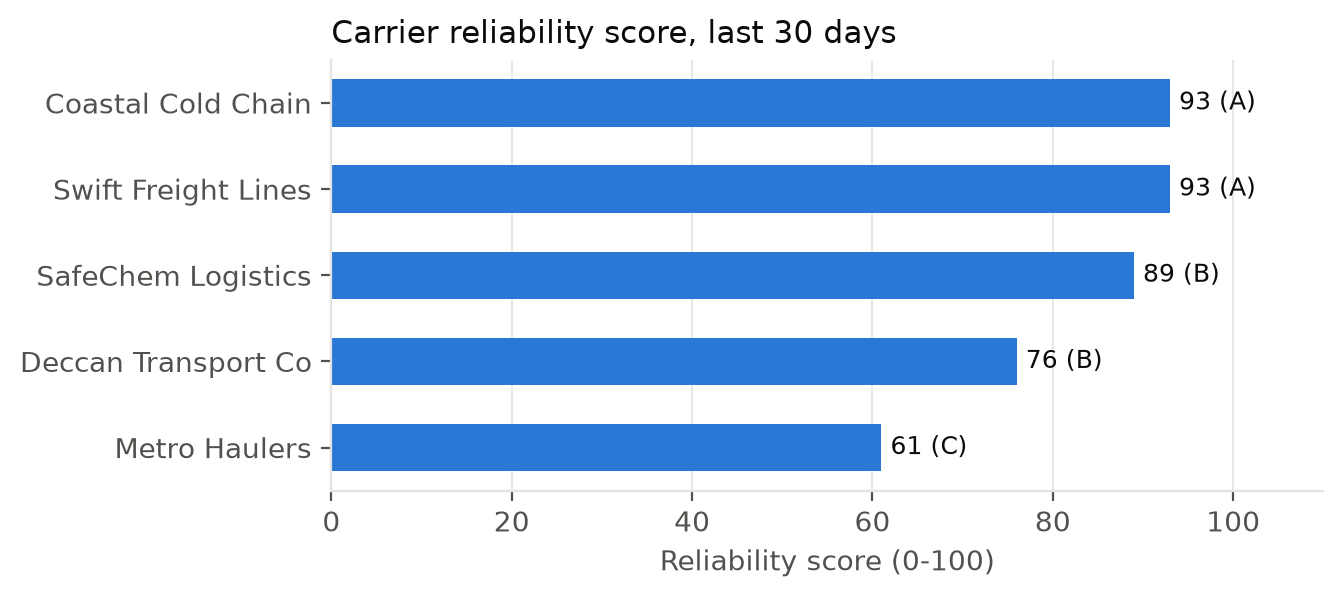
\includegraphics[width=0.85\textwidth]{fig_carrier_reliability.png}
\caption{Carrier reliability scores computed by the system}
\label{fig:rel}
\end{figure}

Figure~\ref{fig:rel} shows how the scorecard separates carriers: Swift Freight Lines and Coastal Cold Chain score 93 (tier A) with on-time rates above 90\%, while Metro Haulers scores 61 (tier C) with a 58\% on-time rate and the most no-shows. These differences are exactly the input a procurement team needs for carrier selection and performance clauses.

\begin{figure}[H]
\centering
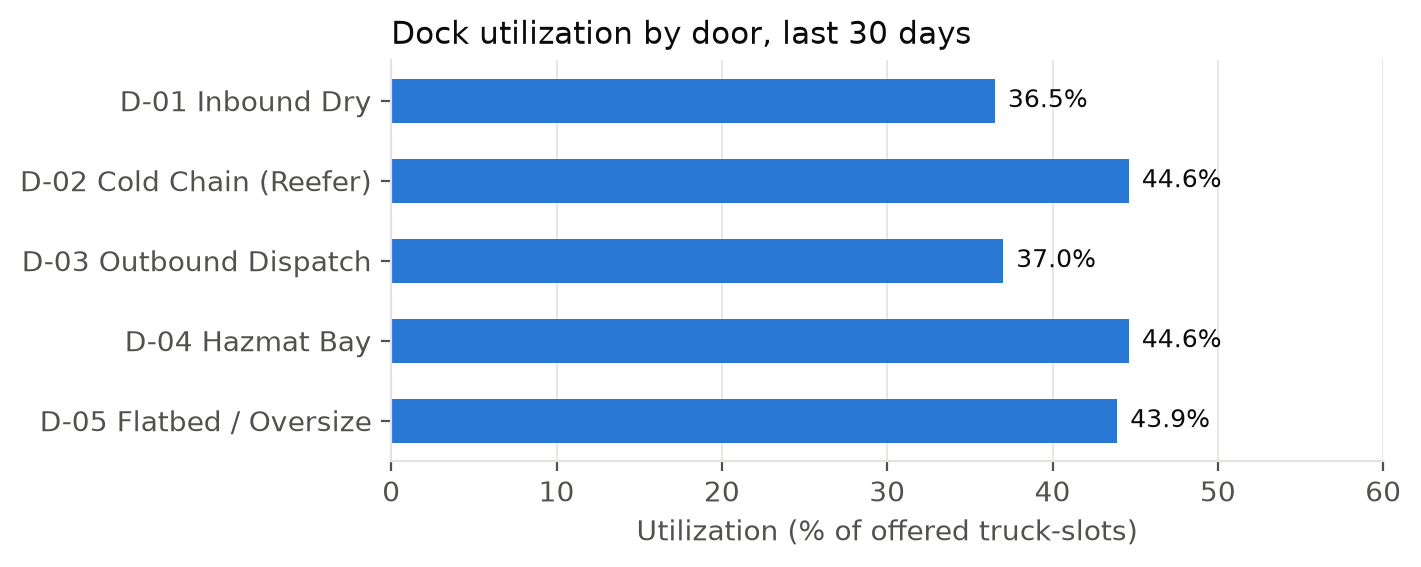
\includegraphics[width=0.85\textwidth]{fig_dock_utilization.png}
\caption{Utilisation by dock door}
\label{fig:dockutil}
\end{figure}

Single-capacity specialised doors (reefer, hazmat and flatbed, about 44--45\%) are relatively busier than the two-truck general doors (about 37\%), suggesting that specialised capacity, not total capacity, would become the constraint first as volume grows.

\section{Before-versus-After Comparison (Simulation)}
To estimate the effect of appointment scheduling on yard congestion, a discrete-event simulation \cite{law2015} was run (script \texttt{docs/analysis/make\_figures.py}). The model represents one DC day from 07:00 to 19:00 with six identical dock doors and 60 trucks; handling time is triangular (25, 40, 55 minutes) plus 5 minutes turnover; trucks are served first-come-first-served at the first free door. Sixty days were simulated for each scenario with the same random seed.

\begin{itemize}
  \item \textbf{Before (no appointments):} carriers arrive at their preferred time, drawn from a morning peak around 09:30 (55\%) and an afternoon peak around 14:30 (45\%).
  \item \textbf{After (SmartDock):} each carrier books the free 60-minute slot nearest its preferred time, with at most six trucks per slot (one per door), and arrives around the slot start with the punctuality mix observed in the demo data (80\% within $-15$ to $+12$ minutes, 15\% late by 16--55 minutes, 5\% no-show).
\end{itemize}

\begin{table}[H]
\centering
\caption{Simulated yard performance, 60 days per scenario}
\label{tab:sim}
\begin{tabular}{lrrr}
\toprule
\textbf{Metric} & \textbf{Before} & \textbf{After} & \textbf{Change}\\
\midrule
Mean wait from arrival to dock & 19.4 min & 1.0 min & $-95\%$\\
90th percentile wait & 54.9 min & 0.0 min & $-100\%$\\
Maximum wait observed & 116.3 min & 37.7 min & $-68\%$\\
Trucks waiting more than 30 min & 27.7\% & 0.3\% & $-27.4$ pts\\
Peak average yard queue & 7.0 trucks & 0.4 trucks & $-94\%$\\
\bottomrule
\end{tabular}
\end{table}

\begin{figure}[H]
\centering
\begin{subfigure}{0.49\textwidth}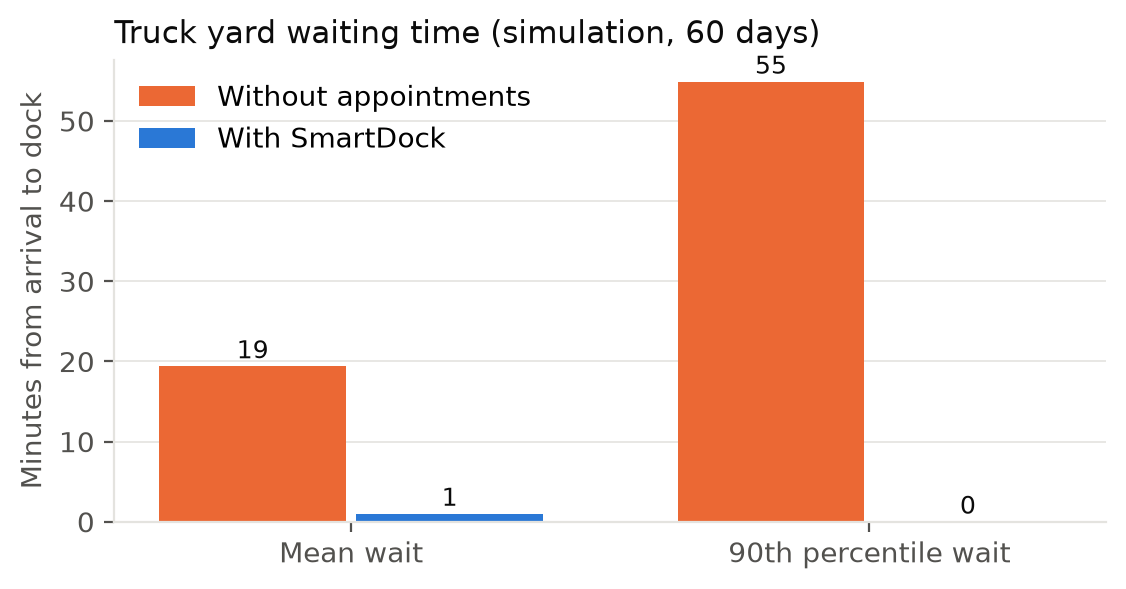
\includegraphics[width=\textwidth]{fig_sim_wait.png}\caption{Waiting time}\end{subfigure}
\hfill
\begin{subfigure}{0.49\textwidth}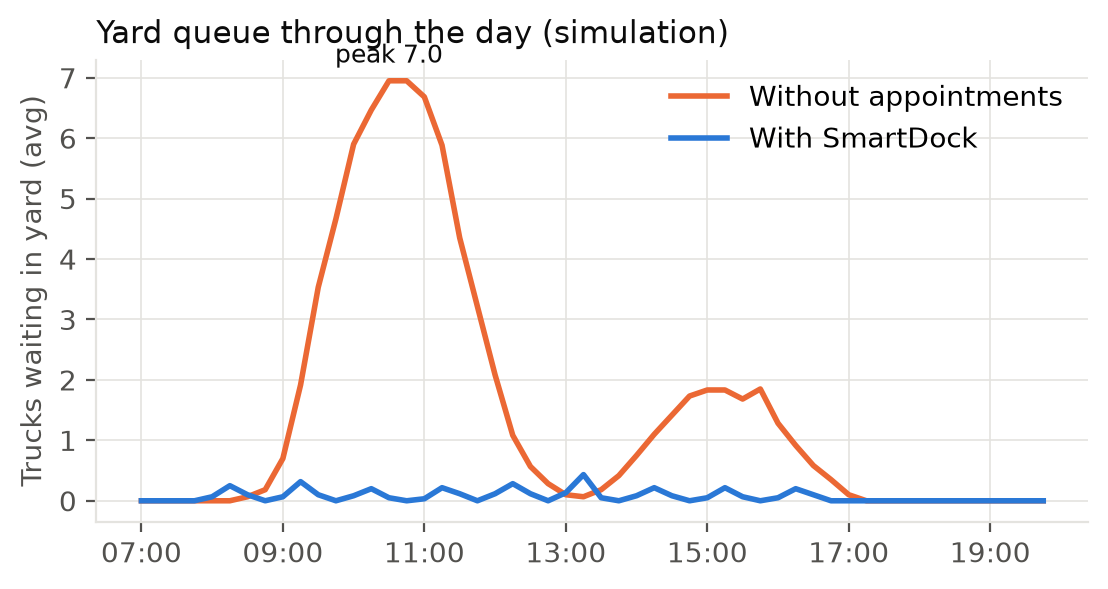
\includegraphics[width=\textwidth]{fig_sim_queue.png}\caption{Yard queue through the day}\end{subfigure}
\caption{Simulated effect of appointment scheduling}
\label{fig:sim}
\end{figure}

\paragraph{Discussion.} With the same docks and the same work, smoothing arrivals removes almost all queueing: the morning and afternoon peaks that create a queue of about seven trucks disappear because capacity is allocated before trucks arrive. The residual waits are caused by late trucks arriving while the next appointment is already at the door, which is precisely what the late-arrival tracking and reliability score are designed to discourage. In money terms, each truck-hour of waiting avoided reduces detention charges, driver hours and idling emissions --- the benefits reported for port appointment systems \cite{giuliano2007,zehendner2014}.

\paragraph{Threats to validity.} The simulation is deliberately simple: identical doors, one truck type, a fixed arrival pattern and perfect slot discipline for punctual trucks. In practice the gain depends on enforcement and carrier compliance \cite{giuliano2007}, on handling-time variability and on how peaky demand really is. The numbers should be read as an indication of the order of magnitude, to be confirmed by a pilot at a real site.

\section{Correctness Result}
The most important technical result is the double-booking experiment (Section~\ref{sec:concurrency}): under 40 simultaneous requests split across two servers, the naive approach admitted 15 trucks into a one-truck slot, whereas SmartDock admitted exactly one (and exactly three into a three-truck slot). For a warehouse this is the difference between a reliable schedule and a schedule that fails exactly at the busiest moments.

\chapter{Benefits, Conclusion and Future Work}

\section{Benefits and Real-World Applications}
\begin{table}[H]
\centering
\small
\caption{Supply-chain impact of SmartDock}
\label{tab:benefits}
\begin{tabularx}{\textwidth}{>{\bfseries\raggedright\arraybackslash}p{2.6cm}X}
\toprule
Dimension & Impact \\
\midrule
Cost & Less truck waiting means lower detention charges and driver overtime; labour can be rostered to the known appointment load (heatmap, busiest hours) instead of covering unpredictable peaks; free and open-source software avoids licence fees. \\
Visibility & Both sides see the same schedule in real time: carriers see free capacity and status; managers see every truck's position (expected, in yard, at door, departed) and live KPIs. \\
Speed & Self-service booking replaces phone and e-mail; the simulation indicates that yard waiting falls from about 19 minutes to about 1 minute per truck; waitlist auto-assignment refills cancelled capacity without manual effort. \\
Traceability & Every appointment carries PO/ASN references, timestamps for each yard event and a complete audit trail, supporting detention disputes, compliance and root-cause analysis. \\
Reliability & Conflict-free scheduling (including dock compatibility and hazmat safety) and a carrier reliability score that creates accountability and supports carrier selection. \\
Sustainability & Shorter queues mean less engine idling and local emissions near the site \cite{giuliano2007}. \\
\bottomrule
\end{tabularx}
\end{table}

\paragraph{Applications.} Distribution centres of retailers and e-commerce companies (inbound supplier deliveries, outbound store or courier pickups); cold-chain warehouses (reefer-only doors and pharma 2--8\,$^{\circ}$C loads); chemical and fuel depots (hazmat bays); third-party logistics (3PL) providers running several client warehouses on one platform (multi-tenancy); manufacturing plants receiving just-in-time inbound parts; and, with minor changes, container freight stations and inland container depots.

\section{Conclusion}
This project designed, implemented, tested and deployed \textbf{SmartDock}, a multi-tenant dock appointment scheduling and yard management system. Mapping back to the objectives:
\begin{itemize}
  \item Multi-tenancy with per-warehouse carrier approval and strict tenant isolation was implemented and verified by automated tests.
  \item A configurable scheduling engine supports slot lengths of 15--90 minutes, turnover buffers, holidays and maintenance windows across time zones.
  \item Loads are matched to doors by direction, trailer type and hazmat certification.
  \item Slot capacity is guaranteed under concurrency across multiple servers; a controlled experiment confirmed the guarantee and demonstrated the failure of the naive approach.
  \item Recurring series, rescheduling and an automatic FIFO waitlist cover realistic carrier needs.
  \item Yard events are digitised, late arrivals and no-shows are detected automatically, and carriers receive a reliability score.
  \item Managers obtain KPIs, heatmaps, scorecards, CSV/PDF reports and a gate sheet; every action is audited and notified.
  \item The system is live on the cloud and passes 58 end-to-end checks.
\end{itemize}
SmartDock shows that a focused information system at the warehouse--transport interface can convert an uncontrolled, phone-based process into a measured, collaborative one, improving cost, visibility, speed and traceability in the supply chain.

\section{Project Links}
\begin{tabular}{@{}ll@{}}
\textbf{Live system} & \url{\LiveURL} \\
\textbf{Source code (GitHub)} & \url{\GitHubURL} \\
\textbf{Demo logins} & \texttt{admin@smartdock.demo}, \texttt{carrier@smartdock.demo} (password \texttt{Demo@123}) \\
\textbf{Run locally} & \texttt{npm run dev:demo} (server) after building the client \\
\textbf{Run tests} & \texttt{npm run verify:critical} (58 end-to-end checks) \\
\end{tabular}

\section{Future Enhancements}
\begin{itemize}
  \item \textbf{AI/ML:} predict no-show probability and arrival delay per carrier, lane and time of day; recommend slots and automatically overbook slightly where no-shows are likely; forecast daily inbound volume for labour planning.
  \item \textbf{Optimisation:} automatic assignment of trucks to doors (minimising yard wait and travel inside the building) and load-dependent slot lengths.
  \item \textbf{IoT and computer vision:} automatic gate check-in by number-plate recognition, RFID or GPS geofencing; dock-door sensors for real dock start and end times; reefer temperature monitoring.
  \item \textbf{Integration:} import purchase orders and ASNs from ERP/WMS, push appointments to TMS, and provide webhooks and a public API for carriers.
  \item \textbf{Mobile app:} a driver app with turn-by-turn directions to the assigned door, digital proof of delivery and live status; installable as a progressive web app.
  \item \textbf{Commercial features:} detention and no-show fee calculation, carrier contracts and service-level agreements, multi-language support.
  \item \textbf{Scalability and operations:} real-time updates with WebSockets instead of polling, caching of analytics, a super-administrator console for 3PL operators, horizontal scaling on a paid plan, and automated CI tests on every commit.
\end{itemize}


\begin{thebibliography}{99}
\addcontentsline{toc}{chapter}{References}

\bibitem{chopra2016} S.~Chopra and P.~Meindl, \emph{Supply Chain Management: Strategy, Planning, and Operation}, 6th ed. Pearson, 2016.

\bibitem{christopher2016} M.~Christopher, \emph{Logistics \& Supply Chain Management}, 5th ed. Pearson, 2016.

\bibitem{ivanov2019} D.~Ivanov, A.~Tsipoulanidis and J.~Schönberger, \emph{Global Supply Chain and Operations Management: A Decision-Oriented Introduction to the Creation of Value}, 2nd ed. Springer, 2019.

\bibitem{gu2007} J.~Gu, M.~Goetschalckx and L.~F.~McGinnis, ``Research on warehouse operation: A comprehensive review,'' \emph{European Journal of Operational Research}, vol.~177, no.~1, pp.~1--21, 2007.

\bibitem{boysen2010} N.~Boysen and M.~Fliedner, ``Cross dock scheduling: Classification, literature review and research agenda,'' \emph{Omega}, vol.~38, no.~6, pp.~413--422, 2010.

\bibitem{giuliano2007} G.~Giuliano and T.~O'Brien, ``Reducing port-related truck emissions: The terminal gate appointment system at the Ports of Los Angeles and Long Beach,'' \emph{Transportation Research Part D: Transport and Environment}, vol.~12, no.~7, pp.~460--473, 2007.

\bibitem{huynh2008} N.~Huynh and C.~M.~Walton, ``Robust scheduling of truck arrivals at marine container terminals,'' \emph{Journal of Transportation Engineering}, vol.~134, no.~8, pp.~347--353, 2008.

\bibitem{zehendner2014} E.~Zehendner and D.~Feillet, ``Benefits of a truck appointment system on the service quality of inland transport modes at a multimodal container terminal,'' \emph{European Journal of Operational Research}, vol.~235, no.~2, pp.~461--469, 2014.

\bibitem{phan2015} M.-H.~Phan and K.~H.~Kim, ``Negotiating truck arrival times among trucking companies and a container terminal,'' \emph{Transportation Research Part E: Logistics and Transportation Review}, vol.~75, pp.~132--144, 2015.

\bibitem{law2015} A.~M.~Law, \emph{Simulation Modeling and Analysis}, 5th ed. McGraw-Hill, 2015.

\bibitem{kleppmann2017} M.~Kleppmann, \emph{Designing Data-Intensive Applications}. O'Reilly Media, 2017, ch.~7 (Transactions: write skew and phantoms).

\bibitem{mongodbtx} MongoDB, Inc., ``Transactions,'' \emph{MongoDB Manual}. [Online]. Available: \url{https://www.mongodb.com/docs/manual/core/transactions/}

\bibitem{owasp2021} OWASP Foundation, ``OWASP Top 10:2021 -- A01 Broken Access Control.'' [Online]. Available: \url{https://owasp.org/Top10/}

\bibitem{react} Meta Open Source, ``React documentation.'' [Online]. Available: \url{https://react.dev}

\bibitem{express} OpenJS Foundation, ``Express -- Node.js web application framework.'' [Online]. Available: \url{https://expressjs.com}

\bibitem{render} Render, ``Blueprint specification (render.yaml).'' [Online]. Available: \url{https://render.com/docs/blueprint-spec}

\end{thebibliography}


\appendix
\chapter{Important Code Snippets}\label{app:code}
The listings below are taken directly from the project source code (\url{\GitHubURL}). Line numbers refer to the original files.

\lstinputlisting[firstline=124, lastline=154, firstnumber=124, caption={Slot grid for one local date: slot length, buffer, holidays (\texttt{server/src/services/scheduling.ts})}, label={lst:grid}]{../../server/src/services/scheduling.ts}

\lstinputlisting[firstline=33, lastline=61, firstnumber=33, caption={Daylight-saving-safe conversion of local slot times to UTC (\texttt{scheduling.ts})}, label={lst:tz}]{../../server/src/services/scheduling.ts}

\lstinputlisting[firstline=99, lastline=114, firstnumber=99, caption={Load--dock compatibility: direction, trailer type, hazmat (\texttt{server/src/models/Dock.ts})}, label={lst:compat}]{../../server/src/models/Dock.ts}

\lstinputlisting[firstline=346, lastline=426, firstnumber=346, caption={Atomic capacity reservation: in-process dock lock and transactional dock write lock (\texttt{scheduling.ts})}, label={lst:reserve}]{../../server/src/services/scheduling.ts}

\lstinputlisting[firstline=58, lastline=73, firstnumber=58, caption={Appointment lifecycle: allowed status transitions (\texttt{server/src/controllers/bookingController.ts})}, label={lst:states}]{../../server/src/controllers/bookingController.ts}

\lstinputlisting[firstline=362, lastline=369, firstnumber=362, caption={Gate check-in: on-time or late arrival (\texttt{bookingController.ts})}, label={lst:checkin}]{../../server/src/controllers/bookingController.ts}

\lstinputlisting[firstline=40, lastline=108, firstnumber=40, caption={Waitlist: first-in-first-out assignment of released capacity (\texttt{server/src/services/waitlist.ts})}, label={lst:waitlist}]{../../server/src/services/waitlist.ts}

\lstinputlisting[firstline=85, lastline=110, firstnumber=85, caption={Carrier reliability score (\texttt{server/src/services/reliability.ts})}, label={lst:score}]{../../server/src/services/reliability.ts}

\lstinputlisting[firstline=18, lastline=47, firstnumber=18, caption={Background job: automatic no-show detection (\texttt{server/src/services/jobs.ts})}, label={lst:jobs}]{../../server/src/services/jobs.ts}

\lstinputlisting[firstline=71, lastline=118, firstnumber=71, caption={Per-request tenant and warehouse-access control (\texttt{server/src/middleware/authMiddleware.ts})}, label={lst:access}]{../../server/src/middleware/authMiddleware.ts}


\end{document}
